\documentclass[a4paper,12pt]{report}
\usepackage{styles/report_format}
\usepackage[style=ieee]{biblatex}
\addbibresource{references.bib}
	
\renewcommand{\labelenumi}{(\roman{enumi})}

\usepackage{amsmath, amsthm, amssymb}
\usepackage[bottom]{footmisc}
\usepackage{graphicx}
\usepackage{longtable}
\usepackage{algorithm}
\usepackage{algorithmic}
\usepackage{subfig}

% Directory of figures
\graphicspath{{figures/}}

% Times New Roman, Requires XeLaTeX or LuaLaTeX
\RequirePackage{fix-cm}
\usepackage{fontspec}
\setmainfont{Times New Roman}


% Numbering at bottom
\usepackage{fancyhdr}
\pagestyle{fancy}
\fancyhf{}% Clear page header/footer
\renewcommand{\headrulewidth}{0pt}% No header rule
\fancyfoot[C]{\thepage}

% Page Margins
\usepackage[top=3.5cm,bottom=2cm,left=3.5cm,right=2cm]{geometry}

% Prevent hypanated words
%\hyphenpenalty=100000

% COVER PAGE parameters
\title{Multi-Model Evaluation of Blackjack Strategies}
\turkcebaslik{Blackjack Stratejilerinin Çok Modelli Değerlendirmesi}
\author{Deniz Genco Atilla}
\subyear{2024}

% APPROVED BY PAGE parameters
\supervisor{Assist. Prof. Dr. Dionysis Goularas}
\examineri{Assist. Prof. Dr. Esin Onbaşıoğlu}
\examinerii{Prof. Dr. Sezer Gören Uğurdağ}
\dateofapproval{.../.../2021}

\begin{document}
\pagenumbering{roman}

% COVER PAGE

\makecoverpage
    
% BLANK PAGE
\clearpage\mbox{}
\clearpage    
\addtocounter{page}{-1}
    
% APPROVAL PAGE
\makeapprovalpage

% ACKNOWLEDGEMENTS PAGE
\begin{acknowledgements}
First of all, I would like to express my deepest gratitude to my advisor, Mr. Onur Demir. His guidance and insightful feedback throughout my project played a very important and effective role in my progress on the project.

I am also grateful to my family for their endless support and love. To my family, who always believed in me and encouraged me to pursue my dreams, your sacrifices and unlimited faith formed the basis of my success.
\end{acknowledgements}

% ABSTRACT PAGE
\begin{abstract}
The project aims to explore and compare the performance of multiple Blackjack-playing models, each employing distinct strategies. These models include brute force, basic strategy chart with/without card counting, Historical Data analysis, reinforcement learning-based decision-making. The project evaluates the effectiveness of each model in terms of win rate, average return, risk management, and adaptability through extensive simulations and evaluations. The findings will highlight the strengths and weaknesses of each playing method, providing valuable insights into the efficacy of different Blackjack strategies.
\end{abstract}

% ÖZET PAGE
\begin{ozet}
Bu proje, her biri farklı stratejiler kullanan birden fazla Blackjack oynama modelinin performansını karşılaştırmayı amaçlamaktadır. Bu modeller arasında kaba kuvvet modelleri, temel strateji çizelgesine bağlı kart saymali ve kart saymasını içermeyen modeller, geçmiş veri analizi yapan bir model, pekiştirmeli öğrenme tabanlı karar veren bir modelyer almaktadır. Proje, kapsamlı simülasyonlar ve değerlendirmeler yoluyla her modelin kazanma oranı, ortalama getiri, risk yönetimi, zaman verimliliği ve uyarlanabilirlik açısından etkinliğini değerlendirmektedir. Bu çıkarımlar, her bir modelin güçlü ve zayıf yönlerini vurgulayarak farklı Blackjack stratejilerinin etkinliği hakkında değerli bilgiler sağlayacaktır.
\end{ozet}

% TABLE OF CONTENTS
\tableofcontents

% LIST OF FIGURES
\listoffigures

% CONTENT
\chapter{INTRODUCTION}
\label{chapter:introduction}
\pagenumbering{arabic}

This report aims to systematically explore and evaluate the performance of various Blackjack-playing models. The models under investigation include brute force methods (always hit, always stand and random hit/stand), adherence to basic strategy charts, analysis using Historical Data, reinforcement learning, and card counting techniques. with the aid of detailed simulations and comprehensive evaluations: win rate, average return, time efficiency, and adaptability. This analysis will provide valuable insights into the strengths and weaknesses of different Blackjack strategies, contributing to a deeper understanding of their practical applications.

Blackjack, also known as 21, is one of the most famous card games in existence. Blackjack, which has its roots in the 16th century, has developed and changed since then and has taken its current form.

Before introducing the historical background of Blackjack, it is high time to become more familiar with some key terms often mentioned in this report. Understanding these terms will give a foundation for understanding the various strategies and models that would be taken up in the later parts.

\section{Terms}
\begin{itemize}  
\item \textit{Blackjack}: A card game where the player tries to hold cards that have a value close to 21 but do not go over. The players are playing against the house dealer, not other players. However a misplay in the table done by another player can ruin other hands as well.

\item \textit{Basic Strategy}: The mathematically derived strategy provides an optimal way to play every possible hand in a game of Blackjack, depending on the total in the player's hand and the dealer's visible card. This strategy is meant to minimize the house edge.

\item \textit{House Edge}: The mathematical expectation a casino has over its players, realized as a percentage of the player's original bet and is the average gross profit the casino will likely make from each bet. This house edge ensures that a casino will always profit in the long run.

\item \textit{Card Counting}: A strategy to search the high-to-low card ratio to be dealt in the remainder of the deck. The player hopes to gain an advantage by knowing the likelihood of being dealt good cards.

\item \textit{High Cards}: 10 and over, including 10, Jack, Queen, King, Ace, have a value of 10. These cards place the player in an advantaged position of hitting Blackjack (being an Ace and a value 10 card) and improving the likelihood of strong hands.

\item \textit{Low Cards}: The six and below (2, 3, 4, 5, 6) valued cards are generally less favorable to the player; however, sometimes they can help to avoid busts and even build a strategy towards making a hand without going over 21.

\item \textit{Historical Data Analysis}: Involves the analysis of historical data regarding past game outcomes and player decisions to get possible patterns and extract strategies. It relies on datasets that involve a large number of games played.

\item \textit{Win Rate}: The percentage of games a player or model has won versus some number of games played. It is a critical measure in assessing exactly how good a given Blackjack strategy is likely to perform.

\item \textit{Average Return}: The average amount of money won or lost per game, calculated over many games. It gives one an idea of the profitability of a Blackjack strategy.
\end{itemize}


\section{History of Blackjack} The origin of blackjack is still debated; the most popular belief is that it originated in French casinos around 1700 due to its mention in Cervantes' novel Don Quixote, which dates to the late 16th/early 17th century. At that time, the game was called 'Vingt-et-un', which means 21 in French. On the other hand, there are also those who argue that the Romans once played a game similar to 21 with wooden blocks. In the 18th century, when Blackjack became popular in casinos, casinos created 'special bets' to attract more players to the game, one of these was ,which gave the game its current name, was 10:1 (paying 10 times the stake for each bet), where a player had to draw an ace with a black jack of clubs or spades.


\subsection{Blackjack from eyes of Mathematicians} Over the years, Blackjack has attracted significant attention from mathematicians and researchers who have uncover the best strategies for winning. One of the most notable contributions came from Edward O. Thorp, who developed the basic strategy\cite{book:1} and introduced card counting in his groundbreaking book, "Beat the Dealer," published in the 1960s. Thorp's work revolutionized the way Blackjack is played, providing players with systematic methods to reduce the house edge. Following Thorp, many researchers and enthusiasts have continued to develop and refine various strategies to enhance gameplay. These include complex card counting systems, simulation-based approaches, and the application of artificial intelligence and machine learning to optimize decision-making in the game. The ongoing evolution of these strategies reflects the game's dynamic nature and the continuous quest for improved methods of play.\cite{paper:5}

\section{Research Motivation} The aim to develop optimal strategies for blackjack has been in interest of mathematicians for long time. Despite the simplicity of the game, the interplay of probability and strategies creates a complex challenge that has fuelled extensive researchs. The rise of computational tools and artificial intelligence has opened new ways to explore these challenges and enabled the development of sophisticated models capable of simulating and analysing thousands of game scenarios.

This study was motivated by the desire to comprehensively evaluate and compare the effectiveness of various Blackjack playing models. Traditional strategies such as Edward O. Thorp's basic strategy and card counting have proven their worth over the years. However, newer approaches that machine learning and Historical Data analysis promise to offer new insights and potentially superior performance. Understanding the strengths and weaknesses of these various strategies is crucial for practical applications.

\section{Objective of Study} The primary objective of this project is to explore and compare the performance of several Blackjack-playing models. These models include brute forces, adherence to basic strategy charts, Historical Data analysis, reinforcement learning-based decision-making, and card counting. Through extensive simulations and evaluations, we aim to assess the effectiveness of each model in terms of win rate, average return, time efficiency, and adaptability.

\vskip4\baselineskip

\section{Scope and Limitations}
This study aims to explore and compare the performance of multiple Blackjack-playing models, each employing distinct strategies. The scope of the research includes:

\begin{itemize}
\item \textbf{Model Comparison:} Evaluating five different Blackjack-playing models: brute force models, basic strategy chart based models (with and without card counting), Historical Data analysis, reinforcement learning-based decision-making.
\item \textbf{Performance Metrics:} Assessing the effectiveness of each model based on win rate, average return of invest, risk management and adaptability.
\item \textbf{Simulation:} Creating extensive simulations to generate a large dataset of game outcomes for analysis.
\item \textbf{Strategy Analysis:} Analyzing the strengths and weaknesses of each strategy, providing insights into their practical applicability and profitability.
\end{itemize} 

While this project aims to provide an analysis of various blackjack playing models, it is crucial to acknowledge there are limitations that may impact the findings and their applicability. The following are some of the limitations: 

\begin{itemize}
\item \textbf{Simulation Environment:} The simulations are ran in a controlled environment that may not fully capture the complexities and variances of live casino play. Factors such as human error, psychological influences, and real-time decision-making are not considered.

\item \textbf{Model Assumptions:} Each model relies on specific assumptions that may not be universally applicable. For instance, card counting is often predicated on the use of a single deck, double deck or a known number of decks, and assumes certain rules like the dealer standing on a soft 16. These assumptions do not always align with real-world casino practices, where multiple decks are typically used and shuffled frequently, and the rules may vary, such as the dealer hitting on a soft 16, which increases the house edge.

\item \textbf{Data Availability:} The Historical Data analysis model relies on the availability and accuracy of past game data. Any inaccuracies or biases in the data can affect the model’s performance and conclusions.
\end{itemize} 

\section{Problem Definition}
The project aims toward giving an objective for various playing and analysis strategies in the game of blackjack by simulation, with the end game being able to identify the best approach that provides maximum profit for players. Therefore, it is multi-dimensional in designing, implementing, and evaluating many models because of the unique strategies of implementing games during decision-making, brute force strategies, basic strategy with and without counting, historical data, and reinforcement learning models. Adapting these models will make it a comprehensively applicable tool for blackjack strategy analysis that combines detailed simulation with an intuitive interface to provide insights into the comparison between effective differences in playing strategies.

\section{Requirements} This section outlines the essential requirements for the project, detailing the project's objectives, the methodology for implementation and the evaluation tests to measure its success.

\subsection{Project Objectives}
\begin{itemize}
\item \textbf{Develop and Compare Blackjack Models:} Implementing multiple blackjack models such as brute force models (always hit, always stand, random hit/stand), basic strategy, Historical Data analysis, reinforcement learning-based decision-making, and card counting.
\vspace\baselineskip
\item \textbf{Simulating Extensive Gameplay:} Running a great amount of simulations in order to create a comprehensive dataset of game outcomes.
\vspace\baselineskip
\item \textbf{Evaluate Performance Metrics:} Assess each model based on some metrics such as win rate, average return of invest, risk management and time efficiency.
\vspace\baselineskip
\item \textbf{Analyze and Interpret Results:} Provide insights into the strengths and weaknesses of each model and by visualizing these insight creating a better understanding in which model provides what.
\end{itemize}
\vspace\baselineskip

\subsection{Implementation Methodology}
\begin{itemize}
\item \textbf{Model Development:} Implement the Blackjack-playing models using Python. The models include brute force strategies such as always hit, always stand, and random hit/stand, as well as strategies based on Historical Data and basic strategy.
\vspace\baselineskip
\item \textbf{Simulation Execution:} On the playfield of solid pseudo-random number generators, it is possible to reproduce realistic game conditions. As default behavior, each model will be tested for 2000 simulations, using six decks in each simulation. It's possible to set the number of simulations using parameters.
\vspace\baselineskip
\item \textbf{Data Analysis:} Compare the performance of each model by scrutinizing the statistical analysis. You can analyze the critical metrics of win rate, average return, risk management, and adaptability.
\vspace\baselineskip
\item \textbf{Documentation and Reporting:} All the methodologies, implementations, and results must be well documented. Use visualization tools to make the findings evident, for example, using charts and graphs to show the comparative performance of the models.
\end{itemize}


\chapter{BACKGROUND}
\label{chapter:background}

In this chapter, we will explore the foundational concepts and advancements that have shaped modern blackjack strategies. We will discuss various previous works conducted in this field over different periods and models.

\section{Previous work}
There are numerous strategies to Blackjack, each developing over time as the players try to outsmart the house. At first, players developed mathematical and statistical methods to optimize their play. With time, card counting techniques that were also based on mathematical applications became popular to further optimize the player's chances. More complicated and modern technologies nowadays, and most especially within the framework of machine learning, bring even more potential to optimize Blackjack strategies. Here is some previous work on basic plan, card counting, and machine learning:

\begin{itemize}
\item {\textbf{Basic Strategy}}

The concept of an ideal strategy in Blackjack is not new and has inspired study for many years. The foundation on which the present basic strategy rests was that published in essence by Baldwin, Cantey, Maisel, and McDermott in the classic 1956 paper, "The Optimum Strategy in Blackjack." A mathematically based strategy for players to use to minimize the house edge and gamblers to play with the best odds possible was defined in this paper. \cite{paper:2}.

Further advancements were made by A. R. Manson, A. J. Barr and J. H. Goodnight in "Optimum Zero-Memory Strategy and Exact Probabilities for 4-Deck Blackjack," published in 1975. This research provided a detailed analysis of optimal strategies for multi-deck Blackjack games, which are more commonly used in casinos \cite{paper:3}.

\item {\textbf{Card Counting}}

Card counting, a technique that involves tracking the ratio of high to low cards remaining in the deck, was popularized by Edward O. Thorp in his book "Beat the Dealer."\cite{book:1} The effectiveness of card counting as a strategy was further explored and mathematically validated in subsequent studies.

In 1973, I. Archer published his book, "The Archer Method of Playing 21,"\cite{book:2} where he describes in detail the developed system, which later became known as the "Archer Method" and is the first published card counting system for playing blackjack. In the Archer method, the player keeps track of the ratio of high cards to low cards in the deck and bets either more or less according to his calculated advantage and optimal strategy. This book gave a mathematical foundation to the Archer Method, and he offered practical advice on how it might be applied at the casino tables playing blackjack.

In J.T. Gollehon's book "Pay the Line,"\cite{book:3} published in 1987, many essential blackjack playing strategies are treated in-depth, including the chapters on card counting techniques. The book covers all the fundamentals of blackjack, basic strategy, and more sophisticated ideas like team play and shuffle tracking. It can be used as a valuable closet reference that will help both novice and well-seasoned blackjack players find an edge when playing against the casino.

\item {\textbf{Machine Learning}}

A significant contribution to the field was made in 1992 by S. Yakowitz and M. Kollier, a paper that provided an in-depth analysis of the efficacy of card counting using machine learning techniques.\cite{paper:6} Their work transcribed the search for optimal counting strategies in blackjack into the task of finding a global minimum of a multi-modal discontinuous objective function based on noisy measurements. This approach, termed 'stochastic minimization,' required minimal modeling or understanding of the problem structure. It contrasted with earlier analyses by Thorp, Braum, and others, who relied heavily on combinatorics.

The exploration of different actions and the retention of those that maximize performance become crucial. A notable study by Perez-Uribe, A. and Sanchez, E. explores the use of blackjack as a test bed for neural network-based learning strategies, with a particular focus on reinforcement learning techniques.\cite{paper:7} This research highlights how reinforcement learning allows the system to autonomously develop a strategy by experimenting with various actions, leading to improved performance over time. Performance comparisons with earlier approaches demonstrate the advancements achieved through these modern techniques, offering a fresh perspective on optimizing gameplay in blackjack.

In recent years, the advent of machine learning has introduced new dimensions to Blackjack strategy development. A notable study published in 2012 by Schiller, Marvin R. G.and Gobet, Fernand R. compared cognitive models with AI models in learning Blackjack strategies, highlighting the potential for artificial intelligence to outperform traditional human-devised strategies in certain scenarios. \cite{paper:5}. This research underscores the evolving nature of strategic play in Blackjack, where computational methods are increasingly being employed to optimize decision-making processes.


\end{itemize}


\chapter{ANALYSIS}
\label{analysis}
In this section, we will explore and analyze several key algorithms used in our card game model. These include brute force models, basic strategy models with and without card counting, a Historical Data model, and a reinforcement learning (RL) model. Each algorithm will be described in detail with corresponding pseudocode and diagrams to illustrate their functionalities and implementations. Through this analysis, we aim to understand the strengths and weaknesses of each approach and how they contribute to the overall performance of the model.

\section{Card, Deck and Hand System}
To play a game of Blackjack, cards are essential. Each card has a suit and a color. The colors are traditionally red and black, corresponding to the four suits commonly found in French-suited playing cards: hearts, diamonds, clubs, and spades. The Deck class simulates a standard deck of 52 playing cards. It includes methods for shuffling the deck and dealing cards. It uses \textit{random} built-in library of python in order to shuffle cards. The Hand class represents the hand of a player or house in Blackjack. It keeps a record of the cards in the hand, the total value of the hand and the number of aces.
\vskip\baselineskip
\section{Algorithms}
\label{algorithms}
In this section, we will examine algorithms prepared in four different categories to be simulated. These algorithms include the following: brute force strategies such as always hit, always stand, and random hit/stand; models that play using various basic strategy charts; a model that utilizes card counting in conjunction with basic strategy charts; a model based on Historical Datasets; and a different model employing reinforcement learning machine learning techniques.
\vskip\baselineskip
\subsection{Brute Force}
\subsubsection{Always Hit} 
The "always hit" strategy, as its name suggests, is based on setting a predetermined threshold and continuing to hit (request additional cards) as long as the total value of its hand remains below this threshold. The choice of this threshold is crucial; setting it too low will result in the computer standing with a weak hand, thereby reducing its chances of winning. Conversely, setting the threshold too high increases the risk of the computer busting (exceeding a hand value of 21), which also negatively impacts the win rate. Therefore, fine-tuning this threshold is essential for optimizing the player's performance and maximizing the win rate.

\begin{figure}[H]
\framebox[6.0in]{
\begin{minipage}[b]{5.9in}
\begin{algorithmic}[1]
\REQUIRE player\_hand, deck, AlwaysHitBruteForceSettings
\STATE \textbf{Set} ifHitted $\leftarrow$ False
\WHILE{player\_hand.get\_value() $\leq$ AlwaysHitBruteForceSettings['Threshold']}
    \STATE \textbf{Set} ifHitted $\leftarrow$ True
    \STATE Add a card from the deck to player\_hand
\ENDWHILE
\end{algorithmic}
\end{minipage}}
\caption{Always Hit Algorithm}
\label{alg:always_hit}
\end{figure}

As in Figure \ref{alg:always_hit} shown, while player has a card value below the set threshold, it keeps hitting for more cards.

\subsubsection{Always Stand} 
The "always stand" strategy, involves the computer standing (not requesting additional cards) regardless of the total value of its hand. This strategy is based on a conservative approach, aiming to avoid the risk of busting. However, setting this strategy inherently means the computer might often stand with a weak hand, resulting in fewer wins. Since the computer never takes the opportunity to improve its hand by hitting, this strategy generally leads to a lower win rate, particularly when the initial hand value is low.

Since the "always stand" strategy does not involve hitting, the algorithm for this model does not include any mechanism for adding cards to the player's hand. Instead, the player's hand remains static after the initial deal. Consequently, the algorithm focuses on the dealer's actions, continuing to add cards to the dealer's hand until the dealer reaches the table threshold, similar to other models.

\vskip\baselineskip
\subsubsection{Random Hit/Stand} 
The “random hit/stand” strategy introduces a random possibility decision process into solution. The computer chooses to either hit or stand based on a probabilistic model. This approach imitates a less deterministic playstyle, which in certain situations is reminiscent of the unpredictable decisions of human players. Yet the resolution, since this is random, frequently leads to less than optimal calls, either hitting when it ought to be staying put, or staying put when it ought to be hitting. A major limitation of Genetic Algorithms is that they have a high degree of variability, which often results in unstable results, and therefore a lower win rate that a more systematic model might produce. 

\begin{figure}[H]
\centering
\resizebox{0.8\linewidth}{!}{
\framebox[6.0in]{
\begin{minipage}[b]{5.9in}
\begin{algorithmic}[1]
\REQUIRE player\_hand, deck
\STATE \textbf{Initialize} lastAction $\leftarrow$ []
\WHILE{True}
    \STATE action $\leftarrow$ random choice from ['H', 'S']
    \STATE player\_total $\leftarrow$ player\_hand.get\_value()
    \IF{action == 'H' and player\_total $\leq$ 21}
        \STATE Add a card from the deck to player\_hand
        \STATE Append 'H' to lastAction
    \ELSE
        \STATE Append 'S' to lastAction
        \STATE \textbf{break}
    \ENDIF
\ENDWHILE
\end{algorithmic}
\end{minipage}
}}
\caption{Random Hit/Stand Algorithm}
\label{fig:randomhitstand}
\end{figure}

In Figure \ref{fig:randomhitstand}, we observe that the action is selected from a list containing “Hit” (H) and “Stand” (S). Based on this selection, the corresponding action is executed.

\subsection{Basic Strategy}
\label{basic_strategy}
Basic strategy models develop based on a mathematically derived set of rules formulated to minimize the house edge in Blackjack. These rules, called basic strategy, provide the player with the best action to take in any situation presented, given their hand and the dealer's upcard.

The basic strategy charts graphically illustrate all the optimum plays, given every possible combination of the player's hands and the dealer's upcard. Generally, the charts are in tabular form, with the player's hand values on one axis of the table and the dealer's up-cards on another. The cells of the chart tell the right play for that situation—hit, stand, double down, split, etc.

\vspace{5cm}

\begin{figure}[htbp]
\begin{center}
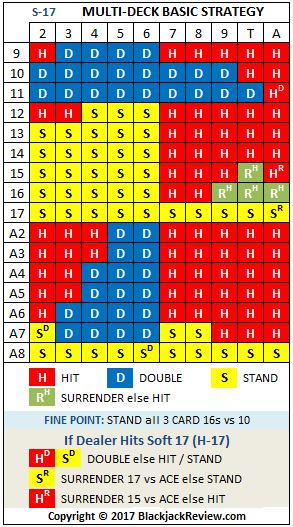
\includegraphics[scale=0.5,keepaspectratio]{figures/BasicStrategy_Multideck.jpg}
\end{center}
\caption{A Basic Strategy chart for multi-deck games}
\label{fig:BasicStrategy_Multideck}
\end{figure}
\vskip\baselineskip

Figure \ref{fig:BasicStrategy_Multideck} contains the basic strategy for multi-deck Blackjack games, indicated in a chart as the optimal decision to be made (Hit, Stand, Double, or Surrender) once the player's total hand value is known (down the left-hand side). The dealer's upcard is shown (across the top). The actions are color-coded: red for Hit, yellow for Stand, blue for Double, and green for Surrender. Players who follow this chart make statistically optimal decisions that keep the house edge to a minimum, making your chances of winning more favorable.


\vskip\baselineskip 
\textbf{General idea of basic strategy models is as follows:}
\begin{itemize}
\item \textbf{Input Parameters:} The input parameters are the value of the player's hand and the dealer's upcard.
\item \textbf{Chart Lookup:} The model refers to the basic strategy chart to determine what the best action is for a specific combination of the player's hand and the dealer's upcard.
\item \textbf{Decision Making:} Possible actions that the model takes, given a recommendation from the chart, include hit, stand, double down, or split.
\item \textbf{Execution:} The model performs the chosen action and updates the hand value in response.
\item \textbf{Repeat:} The process is repeated until the value of the player's hand suggests no more suggested action, e.g., stand or bust.
\end{itemize}

\begin{figure}[H]
\framebox[6.0in]{
\resizebox{0.7\linewidth}{!}{
\begin{minipage}{5.9in} % Adjust the width as necessary
\begin{algorithmic}[1]
\REQUIRE player\_hand, dealer\_hand, deck
\STATE \textbf{Initialize} dealer\_up $\leftarrow$ dealer\_hand.cards[0]
\STATE \textbf{Initialize} action $\leftarrow$ find\_action(player\_hand, dealer\_up) in chart

\WHILE{True}
    \IF{action is Hit}
        \STATE Add a card from the deck to player\_hand
    \ELSIF{action is Double}
        \STATE Add another bet amount to table
        \STATE Add a card from the deck to player\_hand
        \STATE Leave the loop
    \ELSE
        \STATE Leave the loop
    \ENDIF
\ENDWHILE
\end{algorithmic}
\end{minipage}}
}
\caption{Basic Strategy gameplay loop}
\label{alg:basic_strategy_find_action}
\end{figure}

The find\_action function in Figure \ref{alg:basic_strategy_find_action} uses the player's hand value and the dealer's upcard to determine the next action by checking the basic\_strategy table in Figure \ref{fig:BasicStrategy_Multideck}. It retrieves and returns the optimal action for the current game state. In Figure \ref{fig:BasicStrategy_activitydiagram} we can see the activity diagram of basic strategy model:

\begin{figure}[h]
\begin{center}
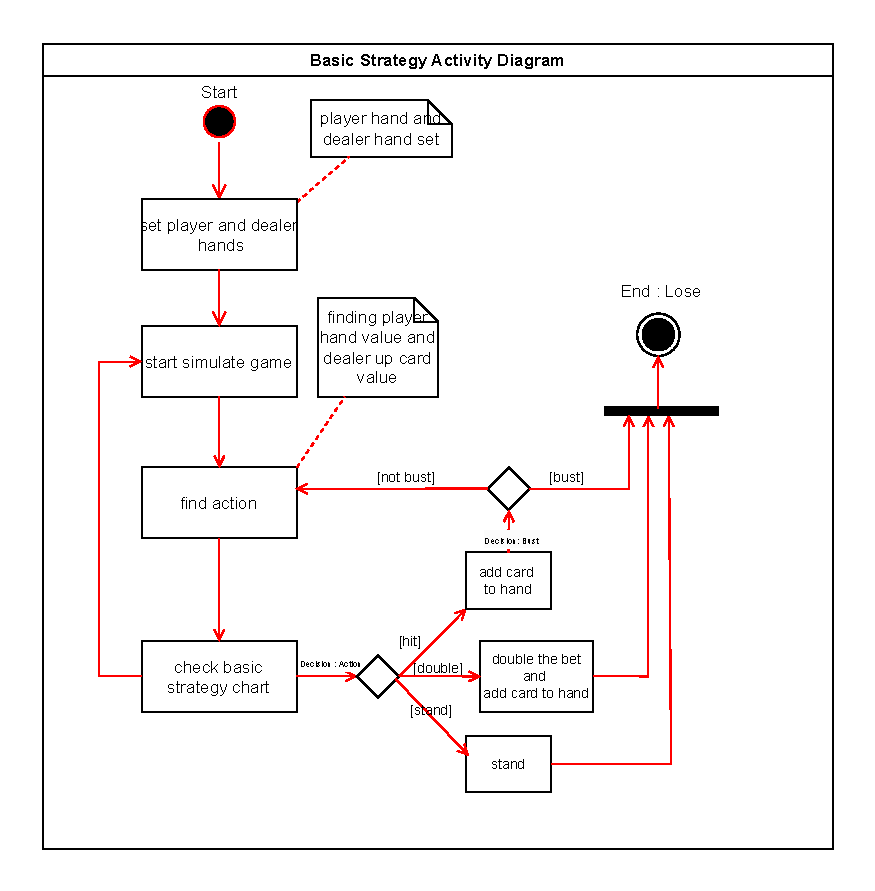
\includegraphics[scale=0.75,keepaspectratio]{figures/basic_strategy_activity_diagram.pdf}
\caption{Basic Strategy Activity Diagram} 
\label{fig:BasicStrategy_activitydiagram}
\end{center}
\end{figure}

The process starts with the initialization of hands for both the player and the dealer Than game simulation initiates based on these values, the appropriate action is identified by referring to a \textit{basic strategy chart}. If the player's hand has not busted, the player must choose between hitting, doubling, or standing. If the decision is to hit, an additional card is drawn and added to the player's hand. If the player doubles hand, the bet is increased, an extra card is drawn, and the hand value is re-evaluated, after this move player cannot take another card from dealer. Alternatively, if the decision is to stand, no further actions are taken, and the turn ends.This cycle continues until a final decision is made. If at any point the player's hand exceeds 21 (busts), the game concludes, and the player loses.

\subsection{Basic Strategy with Counting}
\label{basic_strateg_with_counting}
\textit{Card counting} is a technique used in Blackjack to track the ratio of high cards (10s, face cards, and Aces) to low cards (2 through 6) remaining in the deck. Basic principle is that a deck with a higher part of the cards is advantageous for the player, as it increases the chance of achieving a blackjack and improves odds for doubling down and splitting situations. On the contrary, a deck rich in low cards favors the dealer.

Now let's look at how cart counting works:

\begin{itemize}
    \item \textbf{Assigning Values to Card} : Most counting techniques are using the system Hi-Lo as assigning values to cards.
    \begin{itemize}
        \item \textit{2 to 6} : + 1
        \item \textit{7 to 9} : 0
        \item \textit{10, Jack, Queen, King and Ace} : - 1
    \end{itemize}
    \item \textbf{Running Count} : As cards are dealt, the player keeps a running count by adding or subtracting the assigned values of each card that appears.
    \item \textbf{The True Count} : To account for the number of decks remaining, the player divides the running count to number of decks left to be dealt. This provides the "true count," which is a more accurate measure of the deck's favorability.
    
    \item \textbf{Adjuting the Bet} : The player adjusts their bets from the basic strategy based on the true count. Higher bets are placed when the true count is high (favorable deck), and certain strategy deviations (e.g., hitting, standing, doubling down) are made according to specific index plays derived from the true count.
\end{itemize}

While the basic strategy provides a set of optimal plays for given hands based on the dealer's upcard, card counting enhances this strategy by providing additional information about the rest of the deck. In Figure \ref{alg:running_count}, Figure \ref{alg:update_running_count} and Figure \ref{alg:calcualte_true_count} we can see how to calculate running count, true count and adjusting the bet according to these values.

\begin{figure}[H]
\framebox[6.0in]{
\begin{minipage}[b]{5.9in}
\begin{algorithmic}[1]
\REQUIRE card
\STATE \textbf{Initialize} card\_value $\leftarrow$ card.value
    \IF{card\_value in [2, 3, 4, 5, 6]}
        Increase count by 1
    \ELSIF{card\_value in [10, 11]}
        Decrease count by 1
    \ELSE
        Don't change count
    \ENDIF
\end{algorithmic}
\end{minipage}}
\caption{Counting cards}
\label{alg:running_count}
\end{figure}

In figure \ref{alg:running_count} we can see the part of \textit{Assigning Values to Card} part of the card counting strategy.

\begin{figure}[H]
\framebox[6.0in]{
\begin{minipage}[b]{5.9in}
\begin{algorithmic}[1]
\REQUIRE hand
\FOR{cards in hand}
\STATE \textbf{Initialize} runing\_count $\leftarrow$ runing\_count + count\_card(card)
\ENDFOR
\end{algorithmic}
\end{minipage}}
\caption{Update function for keeping the count of cards}
\label{alg:update_running_count}
\end{figure}

This function in Figure \ref{alg:update_running_count} keeps the ruining count updated for each card dealt on the table. It is called whenever a card drawn from the deck either by a player or dealer.

\begin{figure}[H]
\framebox[6.0in]{
\begin{minipage}[b]{5.9in}
\begin{algorithmic}[1]
\REQUIRE 
\STATE \textbf{Initialize} remaining\_decks $\leftarrow$ amount of remaining cards / 52
\STATE \textbf{Initialize} true\_count $\leftarrow$ runing\_count / remaining\_decks
\end{algorithmic}
\end{minipage}}
\caption{Function for calculating true count}
\label{alg:calcualte_true_count1}
\end{figure}

Finally, the function shown in Figure \ref{alg:calcualte_true_count1} is essential for calculating the true count, which is a critical component of the card counting strategy. To minimize the house edge, the player must adjust their bet size based on the true count. This calculation helps determine the favorability of the remaining decks, allowing the player to make more informed strategic decisions.

\begin{figure}[H]
\framebox[6.0in]{
\begin{minipage}[b]{5.9in}
\begin{algorithmic}[1]
\REQUIRE
\STATE bet\_multiplier $\leftarrow$ maximum of 1 and value of (true\_count multiplied by minimum of remaining\_decks and 1)
\STATE bet\_amount $\leftarrow$ self.minimum\_bet multiplied by bet\_multiplier
\RETURN minimum of bet\_amount and self.money
\end{algorithmic}
\end{minipage}}
\caption{Setting bet size acording to true count}
\label{alg:calculate_betsize}
\end{figure}

It can bee seen in Figure \ref{alg:calculate_betsize} using the true count, the player calculates a bet multiplier. This multiplier is determined as the maximum value between 1 and the product of the true count and the minimum of the remaining decks and 1. The bet amount is then calculated by multiplying the minimum bet with this bet multiplier. Finally, the bet amount is adjusted to ensure it does not exceed the player's available money.

After setting the bet size, the model continues to apply the basic strategy using the new bet size.

\subsection{Historical Data}
The Historical Data model leverages a large dataset of 50 million Blackjack hands \cite{url:1} to determine the optimal actions based on historical outcomes. This dataset, sourced from Kaggle, provides a comprehensive collection of simulated Blackjack hands, reflecting various scenarios and outcomes based on basic strategy. Due to the proprietary nature of casino data, this generated dataset serves as a valuable resource for analyzing and predicting optimal plays in Blackjack.

The dataset includes extensive information on each hand, such as cards remaining, dealer up, initial hand, dealer final, dealer final value, player final, player final value and actions taken. For our purposes, we focus on the columns that capture the initial hand, the dealer's up card, and the action taken. By analyzing these key elements, the Historical Data model can predict the best action for any given hand based on empirical evidence from millions of simulated plays.

The following pseudocode outlines the steps to process the dataset and determine the optimal action based on the initial hand and the dealer's upcard.

\begin{figure}[H]
\framebox[6.0in]{
\begin{minipage}{5.9in}
\begin{algorithmic}[1]
\REQUIRE key
\STATE query $\leftarrow$ "SELECT actions\_taken FROM historical\_data WHERE initial\_hand = ? AND dealer\_up = ? LIMIT 1"
\STATE result $\leftarrow$  Execute query with key[0] and key[1]
\IF{result exists}
    \RETURN result
\ELSE
    \STATE \textbf{USE BASIC STRATEGY}
\ENDIF

\RETURN most\_common\_action\_sequence
\end{algorithmic}
\end{minipage}}
\caption{Pseudocode for Check Next Move}
\label{alg:historical_data}
\end{figure}

As shown in Figure \ref{alg:historical_data}, a database query is created to find the current state in the Historical Data. If the exact game state (e.g., [5, 8] and 8) is found in the Historical Data, it checks for the most repeated action in the dataset and uses it. If it cannot find the exact state, it uses basic strategy to fill the gap in the Historical Data. The reason for using a SQL database in this case is that querying in a SQL database is faster than reading from a CSV file, which is crucial given the importance of speed in our scope.

\subsection{RL Model (Reinforcement Learning)}
\label{RL}
\textit{Reinforcement Learning (RL)} is a type of machine learning where an agent learns to make decisions by performing actions in an environment to maximize the final rewards. Unlike supervised learning, where the model learns from a dataset with labeled examples, RL involves learning through interaction with the environment, receiving feedback in the form of rewards or penalties, and using this feedback to improve future actions.

These are the some of the key steps to create a reinforcement learning model:
\begin{itemize}
    \item \textbf{Defining Environment} : The environment in which the agent operates should be clearly defined, including the states, actions, and reward structure. In blackjack scope; agent is player, states are player's hand vs. dealer's up card, actions are hit, stand and double. Rewarding is determined as winning or losing the current round of blackjack.
    \item \textbf{Initialization the Q-Table} : Q-Table is a table that stores the expected rewards for each state-action pair.
    \item \textbf{Choosing the Hyper-parameters} : Setting values like learning rate (alpha), discount factor (gamma) and exploration rate (epsilon).
    \item \textbf{Implementing a learning algorithm} : There are different learning algorithms differs in model-free RLs and model-based RL. They also splits in each category. In this project Q-learning algorithm from model-free algorithms will be used.
    \item \textbf{Training the model} : Running multiple "episodes" where the agent interacts with the environment and learns from the outcomes.
\end{itemize}

\subsubsection{Explanation of Q-Learning}
Q-learning is a reinforcement learning algorithm that aims to learn the value of the optimal action-selection policy. It uses a Q-Table to store the expected rewards for each state-action pair. The Q-learning algorithm updates the Q-Table based on the Bellman equation:

\begin{equation}
Q(s, a) \leftarrow Q(s, a) + \alpha \left[ r + \gamma \max_{a'} Q(s', a') - Q(s, a) \right]
\label{equation:bellman}
\end{equation}
where:
\begin{itemize}
    \item $Q(s, a)$ is the current value of the state-action pair.
    \item $\alpha$ is the learning rate.
    \item $r$ is the reward received after taking action $a$.
    \item $\gamma$ is the discount factor.
    \item $s'$ is the next state.
    \item $\max_{a'} Q(s', a')$ is the maximum expected future reward for the next state-action pair.
\end{itemize}


Next, let's see how to implement Bellman's equation into the model training code in psudocode:

\begin{figure}[H]
\framebox[6.0in]{
\begin{minipage}{5.9in}
\begin{algorithmic}[1]
\FOR{each episode in range(num\_episodes)}
    \STATE state $\leftarrow$ reset()
    \STATE done $\leftarrow$ False
    
    \WHILE{not done}
        \IF{random number between 0 and 1 is less than epsilon}
            \STATE action $\leftarrow$ random choice from action\_space
        \ELSE
            \STATE action $\leftarrow$ index of the maximum value in q\_table[state]
        \ENDIF
        
        \STATE next\_state, reward, done, \_ $\leftarrow$ step(action)
        
        \IF{next\_state is not in q\_table}
            \STATE q\_table[next\_state] $\leftarrow$ [0, 0, 0]
        \ENDIF
        
        \STATE q\_table[state][action] $\leftarrow$ q\_table[state][action] + alpha * (reward + gamma * maximum value in q\_table[next\_state] - q\_table[state][action])
        
        \STATE state $\leftarrow$ next\_state
    \ENDWHILE
\ENDFOR
\end{algorithmic}
\end{minipage}}
\caption{Pseudocode for Train Model}
\label{alg:train_model}
\end{figure}
\vskip\baselineskip

The train\_model function in Figure \ref{alg:train_model} is for training an agent using the Q-learning algorithm training it in continuous episodes. Inside an episode, an ε-greedy policy dictates the agent's choice of action—exploration of new strategies versus exploitation of known optimal actions. After the action is done, the environment provides feedback which it indicates the next state, reward, and whether the episode is over or not. If the next state is new, it is added to the table of Q-values with initial values. The Q-value for the current state and action pair is updated through the Bellman equation  (Equation \ref{equation:bellman}), where the agent averages the immediate reward and estimate of future rewards. This enables the agent to iteratively update its strategy to maximize the reward.

In the next diagram we can clearly see how train\_model function performs its actions:

\vskip4\baselineskip
\begin{figure}[htb]
\begin{center}
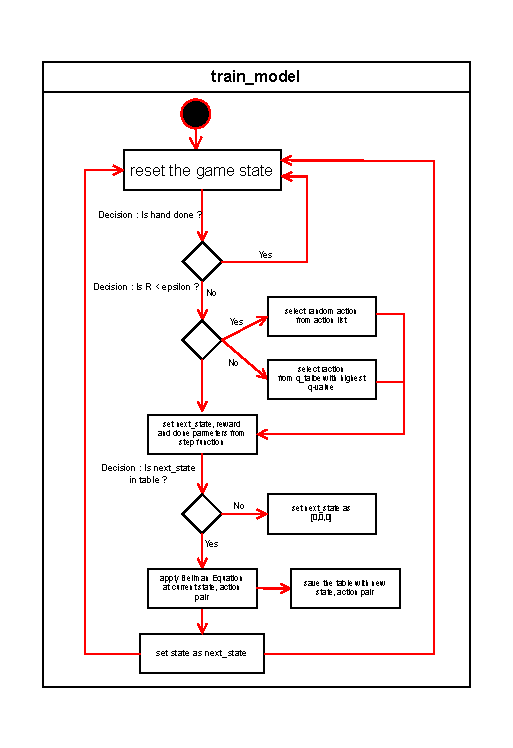
\includegraphics[scale=1.2,keepaspectratio]{figures/train_model_activitydiagram.pdf}
\end{center}
\caption{Train Model Activity Diagram}
\label{fig:train_model_activitydiagram}
\end{figure}

The Figure \ref{fig:train_model_activitydiagram} above illustrates the training process of the reinforcement learning (RL) model for the blackjack application. The process begins with resetting the game state to ensure a fresh start for each episode. The first decision checks if the hand is terminal, which determines if the episode should end. If not, the agent selects an action using an ε-greedy policy, balancing exploration and exploitation. Based on the chosen action, the game state is updated with the new card, and the environment provides feedback, including the next state and reward. The agent then updates the Q-value for the current state-action pair using the Bellman equation, incorporating both the immediate reward and the estimated future rewards. This cycle repeats until the hand is terminal, at which point the episode ends, and the game state is reset for the next episode.

\chapter{DESIGN AND IMPLEMENTATION}
\label{design-and-implementation}
The implementation of the algorithms for the models, user interface, and graphs are all written in Python. The majority of the algorithms utilize the Pandas library for handling data and saving the outputs of the simulations into Excel files for later analysis. For the Historical Data analysis model, SQLite is used to store .csv files into a local database, allowing for faster data searching compared to reading and searching within a .csv file directly. The reinforcement learning (RL) model employs the pickle library for serialization, enabling the saving of the Q-table to a file for future use in determining actions during the blackjack game. Graph creation within the user interface leverages the matplotlib and seaborn libraries, providing robust tools for data visualization. The entire graphical user interface (GUI) is developed using PyQt6, ensuring a rich and interactive user experience.

\section{User Interface}
This section discusses the user interface design, detailing the user interface elements, their functionality, and the benefits they provide to the user.
\vskip\baselineskip
\begin{figure}[htbp]
\begin{center}
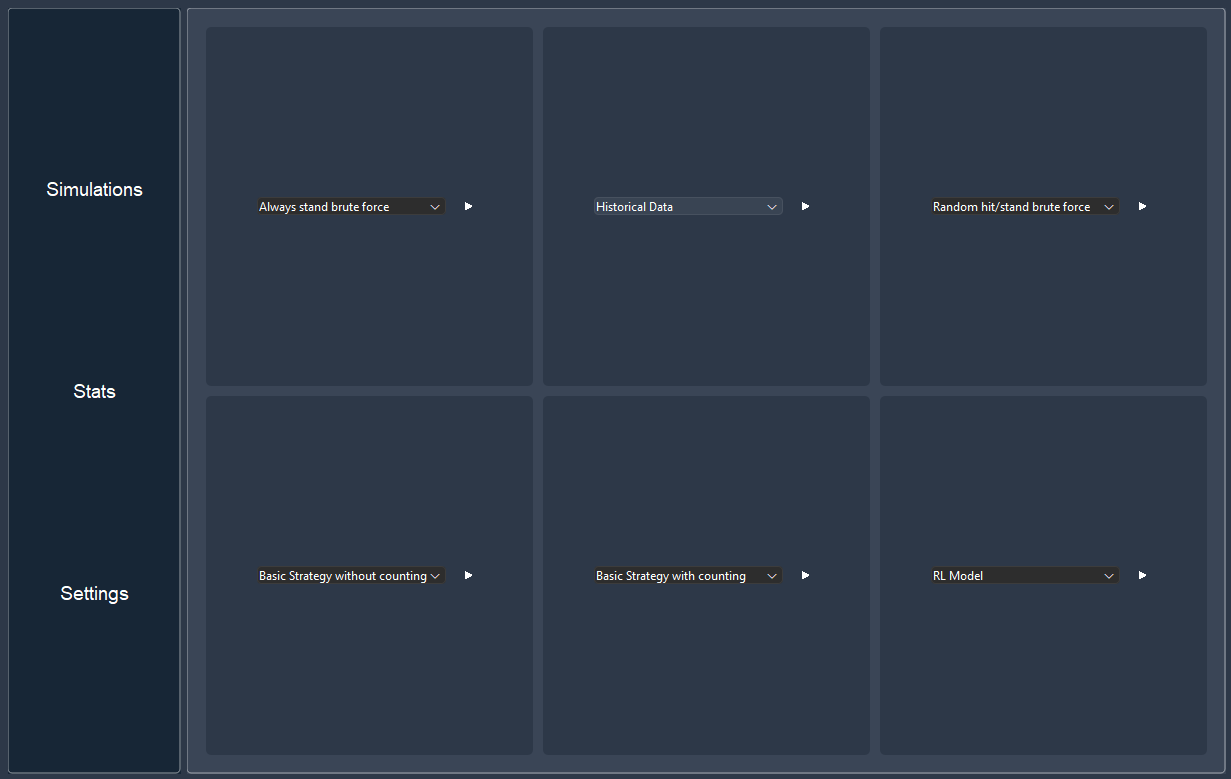
\includegraphics[scale=0.35]{simulation screen.png}
\end{center}
\caption{User Interface : Simulation Screen}
\label{fig:simulation_screen}
\end{figure}

In the simulation screen in Figure \ref{fig:simulation_screen}, users can select up to six models to run concurrently. After selecting the desired model names, pressing the "run" button will create a new thread for each model. The designated algorithms will then be simulated using default settings, unless specific settings have been configured by the user.

\vskip3\baselineskip
\begin{figure}[htbp]
\begin{center}
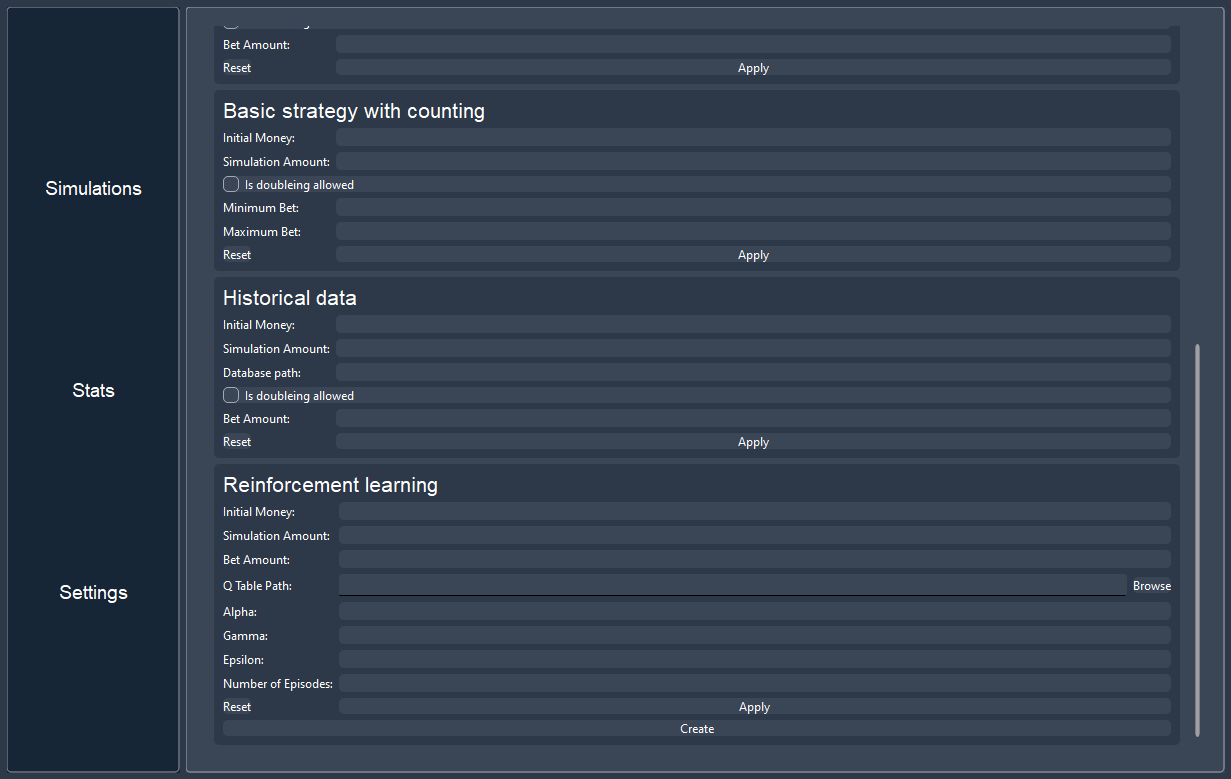
\includegraphics[scale=0.35]{settings screen.png}
\end{center}
\caption{User Interface : Settings Screen}
\label{fig:settings_screen}
\end{figure}

As mentioned above, simulations run with default settings by default. However, users can customize these settings as desired. Each model has different settings, in addition to common settings such as initial money, simulation amount, and bet amount. For example, as shown in Figure \ref{fig:settings_screen}, the Reinforcement Learning model has numerous specific settings. These include simulation settings as well as parameters such as alpha, gamma, epsilon, and the number of episodes for training a model in real-time within the application. To simulate more customized models, users can adjust the desired variables from this settings screen.

\vskip\baselineskip

\begin{figure}[htbp]
\begin{center}
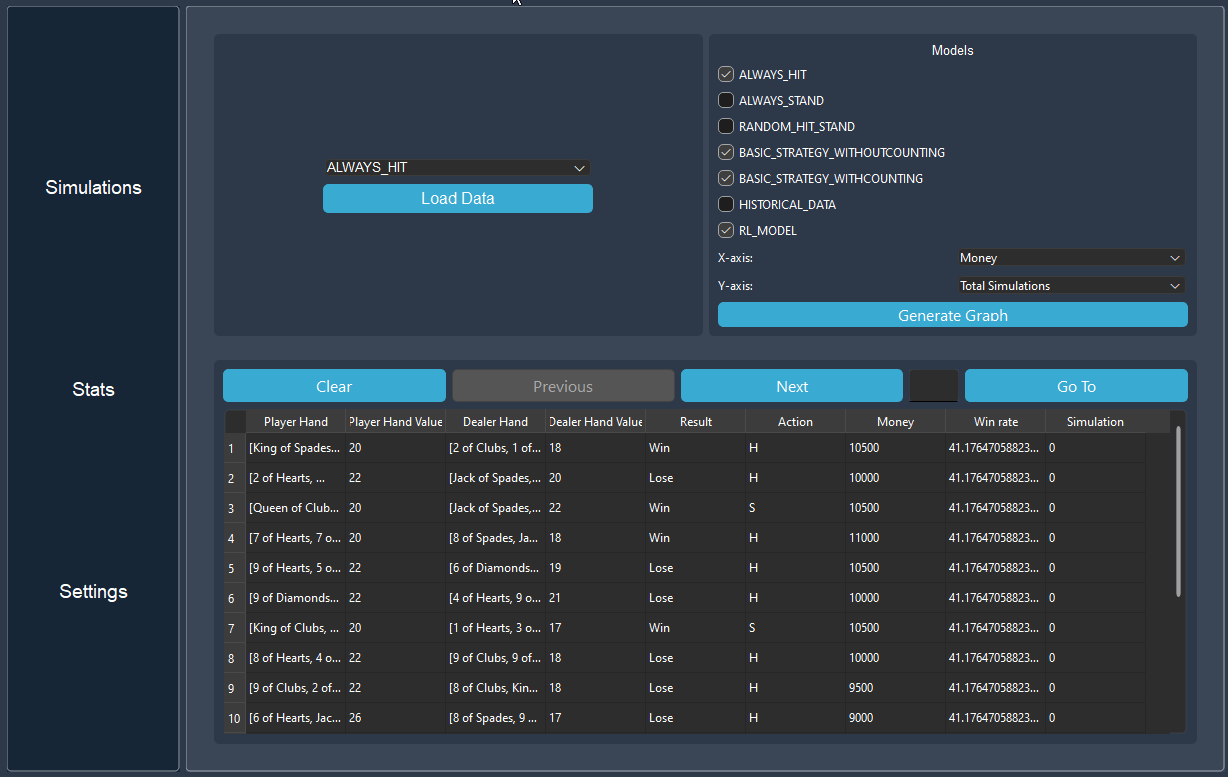
\includegraphics[scale=0.35]{stats screen.png}
\end{center}
\caption{User Interface : Stats Screen}
\label{fig:stats_screen}
\end{figure}

Once the simulations are run, the stats screen displays detailed results (Figure \ref{fig:stats_screen}), including player hands, dealer hands, hand values, results, actions taken, and financial outcomes. Users can navigate through the simulation results, clear the data, and jump to specific simulations using the provided controls.

Additionally, the stats screen offers visualization tools. Users can generate comparative graphs to analyze the performance of different algorithms, with customizable axes and parameters. Graphs are created using matplotlib and seaborn libraries and providing clear and insightful visual representations of the data. This comprehensive analysis capability helps users identify the strengths and weaknesses of each algorithm, facilitating a deeper understanding and enabling the development of optimized blackjack strategies.

\chapter{TEST AND RESULTS}
\label{test-and-results}
In this chapter, the performance and efficacy of the created blackjack playing models will be rigorously compared across various scenarios and dimensions. Each model will be evaluated under different conditions to highlight their strengths and weaknesses. All the data presented in this chapter is directly derived from the application, ensuring accuracy and relevance. Comprehensive graphical representations will be provided for each model, allowing for a visual comparison of their performance. In addition, detailed tables will be included to facilitate an easier and more structured comparison of key metrics.

The analysis will cover several aspects, including win rates, loss rates, average monetary outcomes, and other relevant statistics. These comparisons will help in understanding how each model performs in different game situations, enabling a thorough evaluation of their effectiveness.

\section{Comparing Brute Force Models}
In this section, the brute force models—Always Hit, Always Stand, and Random Hit/Stand—will be compared in terms of win rate, loss rate, money change over win rate, and average return on investment for each model.


All the following algorithms are ran in these parameters:
\begin{itemize}
    \item Initial Money : 10000
    \item Simulation Amount : 2000
    \item Bet Amount : 500
    \item Hit/Stand Threshold (For always hit model) : 17 (by default)
\end{itemize}

\subsection{Always Hit}

The always hit brute force algorithm operates under a straightforward rule: it continues hitting until it reaches a specified threshold. Consequently, in some situations, this model may hit hands that should ideally be stood on, leading to sub-optimal game-play. In the next graph we will see the win rate over the 2000 simulations of always hit brute force model, then we will look into more performance oriented graph such as money x win rate and ROI.

\begin{figure}[h]
\begin{center}
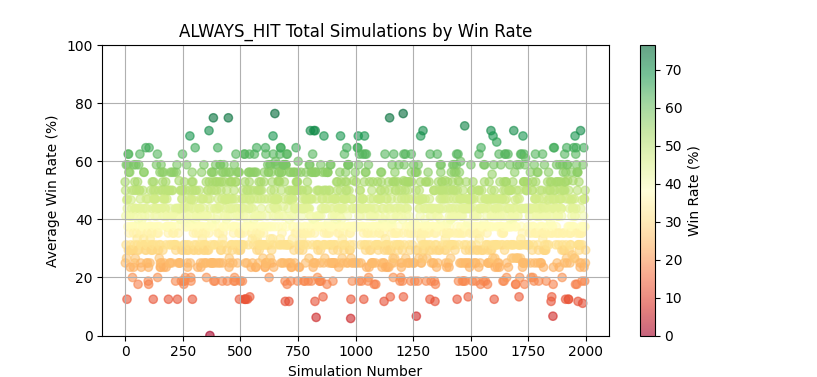
\includegraphics[scale=0.6]{figures/graphs/ah_wr_ts.png}
\end{center}
\caption{Always Hit Model : Win rate x Total Simulations}
\label{fig:ah_wr_ts}
\end{figure}

From the Figure \ref{fig:ah_wr_ts} we can observe a wide range of win rates, with some simulations achieving as high as 80\%, but many clustering around the 25-55\% range. We can classify that 80\%'s and win rates below 20\% as outliers. This variability indicates that while the Always Hit strategy can occasionally perform well, it generally results in a moderate win rate, and there are some outliers at low 20's and high 80'. Now let's look at the money x win rate graph in order to get some intel about profitability of the model.

\begin{figure}[h]
\begin{center}
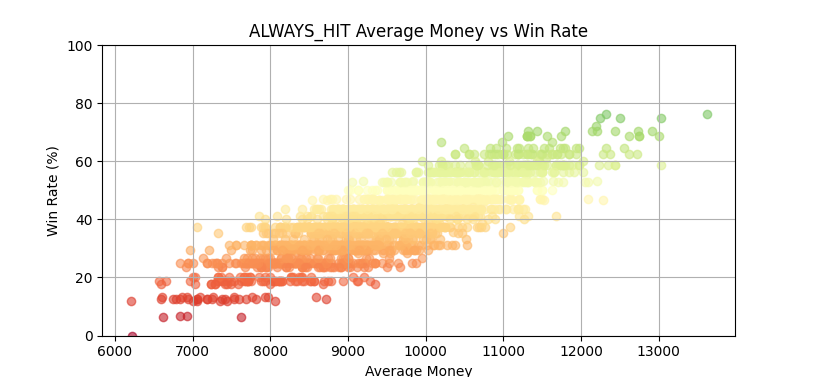
\includegraphics[scale=0.6]{figures/graphs/ah_money_wr_big.png}
\end{center}
\caption{Always Hit Model : Money x Win Rate}
\label{fig:ah_money_wr}
\end{figure}

Since we started simulations at 10000 money, in money x win rate graph (Figure \ref{fig:ah_money_wr}) we can call that the values are right side of the 10000 money, is a profitable simulation, but since the lack of data points on the right side indicates that the always hit model does not consistently guarantee a positive return on investment (ROI). However, within the win rate range of 50-80\%, the model shows a higher density of data points, suggesting that this is the zone where the model is more likely to be profitable. Now let's look at the ROI graph of this model to get better understanding in terms profitability.

\begin{figure}[h]
\begin{center}
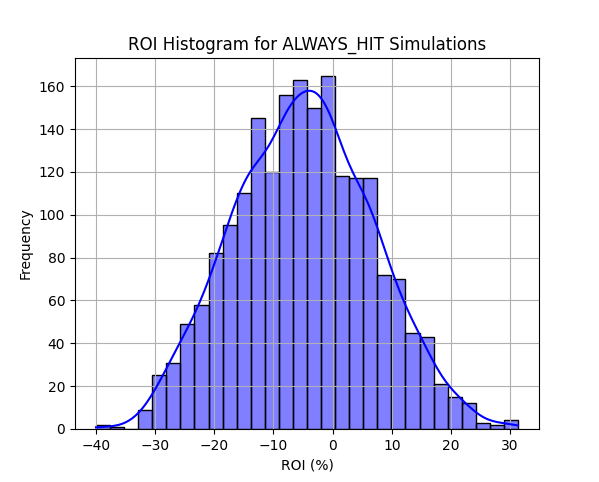
\includegraphics[scale=0.45]{figures/graphs/ah_roi.png}
\end{center}
\caption{Always Hit Model : ROI x Frequency}
\label{fig:ah_roi}
\end{figure}

As shown in Figure \ref{fig:ah_roi}, the graph peaks at an approximate average ROI of -5\%. Notably, the positive ROI section is in the minority, with only about 550 out of 1450 simulations achieving a positive return. This further indicates that the always hit model struggles to consistently generate profits. Since we can set a threshold for the number until which the model will keep hitting, let's compare the thresholds of 16, 17, 18, and 19 with respect to each other:

\begin{figure}[h]
    \begin{minipage}{0.45\textwidth}
        \centering
        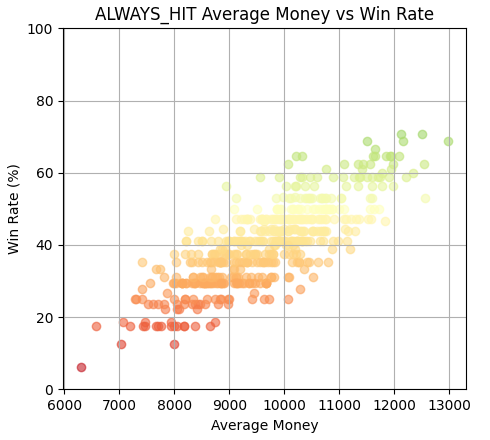
\includegraphics[scale=0.4]{figures/graphs/16.png}
        \label{fig:16}
    \end{minipage}
    \begin{minipage}{0.45\textwidth}
        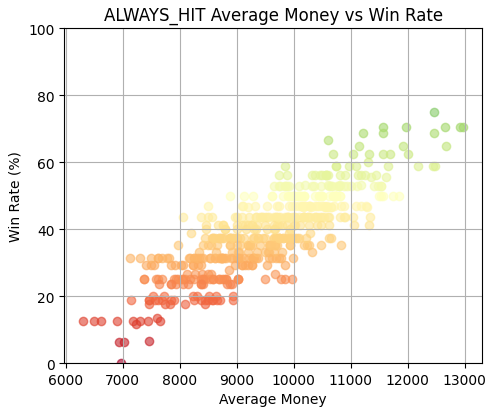
\includegraphics[scale=0.43]{figures/graphs/17.png}
        \label{fig:17}
    \end{minipage}
    \label{fig:16_17}
\end{figure}

\begin{figure}[h]
    \begin{minipage}{0.45\textwidth}
        \centering
        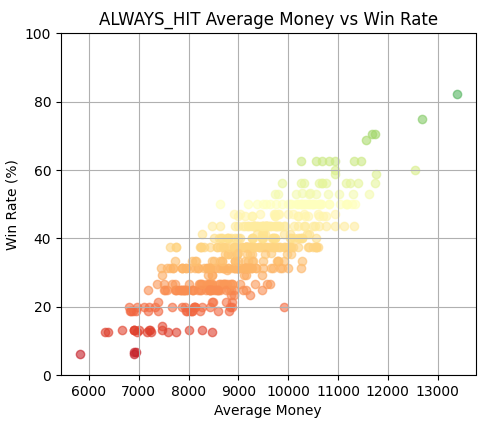
\includegraphics[scale=0.4]{figures/graphs/18.png}
        \label{fig:18}
    \end{minipage}
    \begin{minipage}{0.45\textwidth}
        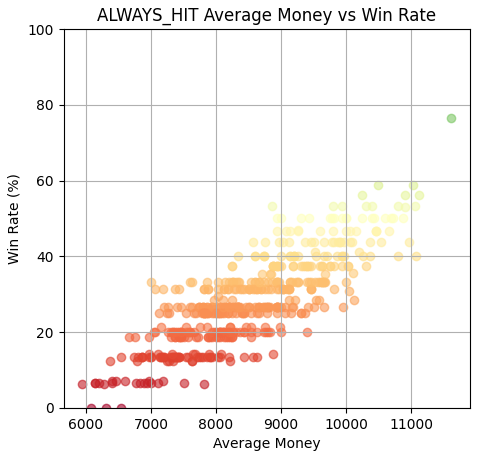
\includegraphics[scale=0.4]{figures/graphs/19.png}
        \label{fig:19}
    \end{minipage}
    \label{fig:18_19}
    \caption{Comprehension of always hit brute force model for thresholds 16, 17, 18 and 19}
\end{figure}
\vskip\baselineskip

In Figure 5.4 we can see that changing the threshold significantly impacts the behavior of the always hit brute force model. In the threshold 19 graph, win rates drastically drop to low 20\% values in many cases, with a limited spread in win rates. On the other hand, at threshold 16, while we observe fewer simulations, there is a notable decrease in win rates below 20\% compared to threshold 17. These graphs clearly show that the threshold setting has a substantial effect on the model's performance. Setting the threshold to 17 or 18 appears to be the most optimal approach, as indicated by the more favorable win rate distributions.


\subsection{Always Stand}
Since always stand model involves the computer standing  regardless of the total value of its hand. There may be performance and profitability since standing on a weak hand may generally lead to a lose. Below the graph of win rate x total simulations graph can be seen:
\vskip2\baselineskip

\begin{figure}[h]
\begin{center}
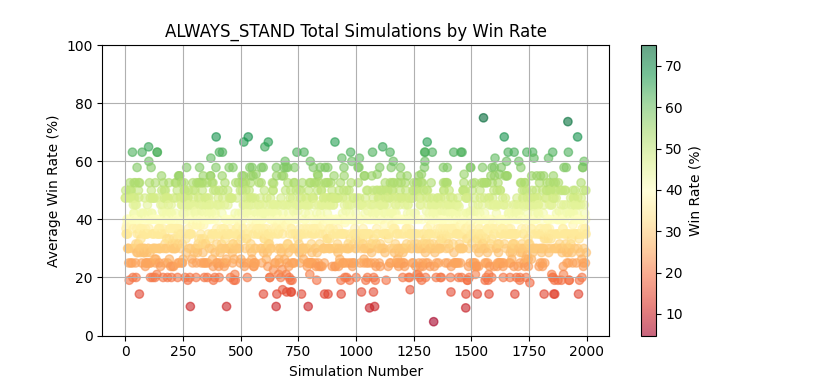
\includegraphics[scale=0.6]{figures/graphs/as_wr_ts.png}
\end{center}
\caption{Always Stand Model : Win rate x Total Simulations}
\label{fig:ah_wr_ts}
\end{figure}
\vskip2\baselineskip

If we compare always stand win rate x total simulations graph in Figure \ref{fig:ah_wr_ts} to the Always Hit model, the high portion of the win rate range is slightly lower, with the majority of simulations falling between 25-50\%, as opposed to 25-55\% for Always Hit. This indicates that the Always Stand strategy tends to perform less consistently at higher win rates, with fewer simulations achieving above 50\%. That concludes always stand model may lead to a lower profitabilty. Now let's check Always Stand model's money x win rate graph to check its lucrativeness.

\vskip2\baselineskip

\begin{figure}[h]
\begin{center}
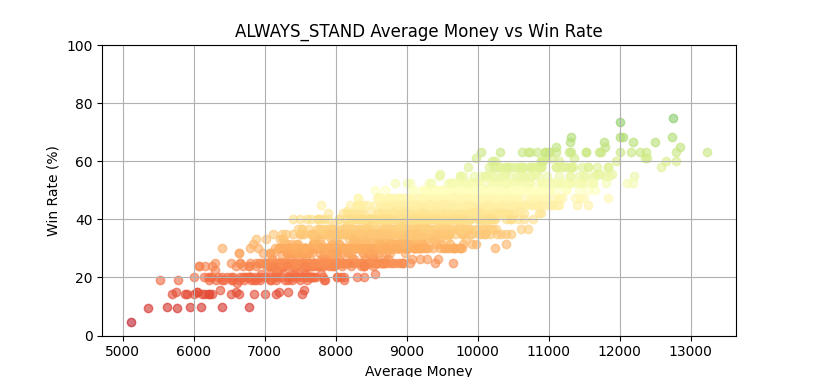
\includegraphics[scale=0.6]{figures/graphs/as_money_wr_big.png}
\end{center}
\caption{Always Stand Model : Money x Win Rate}
\label{fig:as_money_wr}
\end{figure}

Figure \ref{fig:as_money_wr} illustrates the performance of the Always Stand model. It is evident from the graph that the win rates above 60\% are disappeared. The majority of the data points fall within the 20-60\% win rate range, with only a small fraction of these achieving a profit. This indicates that the Always Stand model has limited profitability. We can also see this in ROI graph bellow:

\begin{figure}[h]
\begin{center}
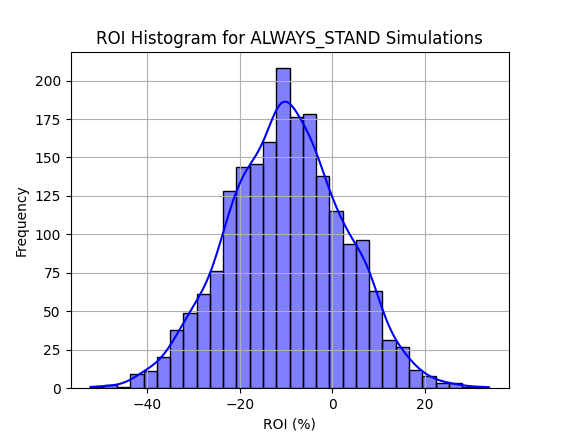
\includegraphics[scale=0.6]{figures/graphs/as_roi.png}
\end{center}
\caption{Always Stand Model : ROI x Frequency}
\label{fig:as_roi}
\end{figure}

Again, it appears in Figure \ref{fig:as_roi} that the number of simulations with a positive ROI is drastically fall. The ratio appears to be approximately 300 to 1700 in terms of +/- ROI's, indicating that the Always Stand strategy results in greater losses compared to the Always Hit strategy.

So far, we have observed that always hitting outperforms always standing. Now, let's explore whether a random selection of actions (hitting or standing) might yield better results.

\subsection{Random Hit/Stand}
Since this approach simulates a more unpredictable style of play, which can sometimes  results in sub-optimal decisions, either hitting when it should stand or standing when it should hit. This variability may result in low performance in terms of ROI and money x win-rate. Let's first delve into the win rate x total simulations graph before mentioning money variable:

\begin{figure}[h]
\begin{center}
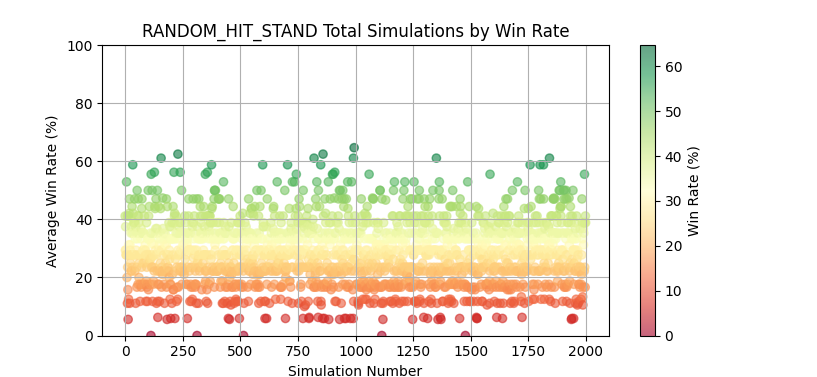
\includegraphics[scale=0.6]{figures/graphs/rhs_wr_ts.png}
\end{center}
\caption{Random Hit/Stand Model : Win rate x Total Simulations}
\label{fig:rhs_money_wr}
\end{figure}

Compared to the Always Hit and Always Stand models we can see that in Figure \ref{fig:rhs_money_wr}, the Random Hit/Stand strategy presents a less consistent performance. The win rates are more spread out, with a noticeable concentration in the 20-40\% range. The highest win rates achieved are slightly above 60\%, but the lower win rates extend down to around 10\%. This variability indicates that the Random Hit/Stand strategy is less reliable, with more simulations resulting in low win rates, and fewer achieving higher win rates. That non-reliabilty shows us that random hit/stand model may not be so reliable to use it as a profitable model. Since we gathered information about win rates, lets dive into how this win rate effects profitability and ROI of the model:

\begin{figure}[h]
\begin{center}
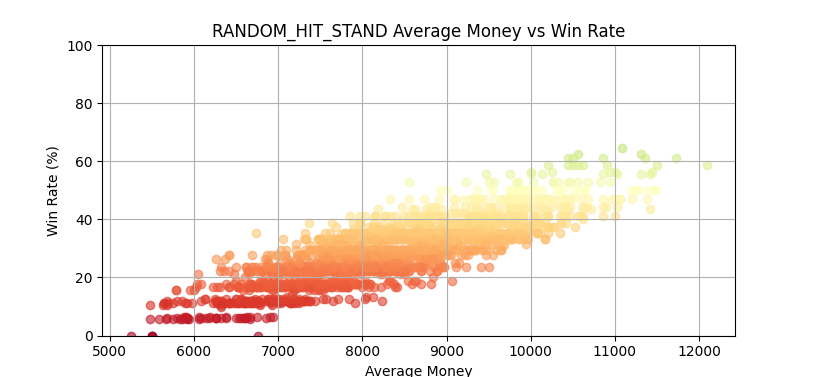
\includegraphics[scale=0.55]{figures/graphs/rhs_money_wr_big.png}
\end{center}
\caption{Random Hit/Stand Model : Money x Win Rate}
\label{fig:rhs_money_wr}
\end{figure}

As expected, selecting random actions results in worse outcomes compared to the other two models. The win rates for this model mostly fall below 55\%, with a significant number of games under 20\% as can be seen from Figre \ref{fig:rhs_money_wr}. Given these results, it is clear that the ROI for this model is also lower than the others. Let's examine the ROI vs. Frequency graph to confirm this:

\begin{figure}[h]
\begin{center}
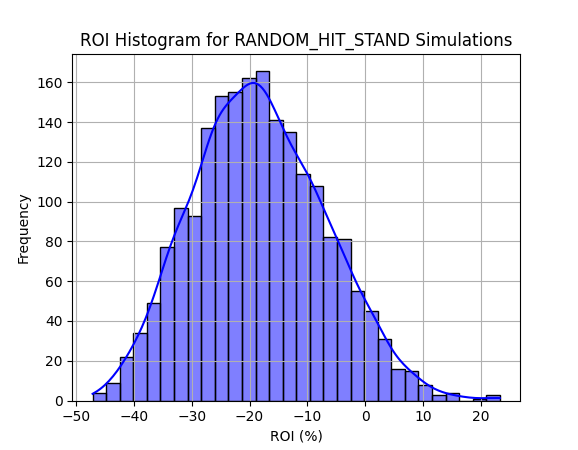
\includegraphics[scale=0.6]{figures/graphs/rhs_roi.png}
\end{center}
\caption{Random Hit/Stand Model : ROI x Frequency}
\label{fig:rhs_roi}
\end{figure}

As Figure \ref{fig:rhs_roi} shows that the ROI has drastically diminished, with the ratio of positive to negative ROI being approximately 100 to 1900. This poor performance indicates that using a random action selection strategy in a game of blackjack is highly inadvisable. In fact, relying on any of the brute force models is generally unfavorable in terms of ROI. 

Therefore, let's set aside our "best" brute force model as Always Hit and proceed to evaluate better models, such as those based on basic strategies and later on models that relies on machine learning.

\section{Comparing Basic Strategy Models}
In this section, we will compare the basic strategy without counting to the basic strategy with counting. Subsequently, we will evaluate the profitability of the better algorithm in comparison to our best brute force model, which is the Always Hit model.

\subsection{Basic Strategy without Counting}
As mentioned earlier in \ref{basic_strategy}, the basic strategy model determines its actions based on a \textit{basic strategy chart}. Let's first check that how well that basic strategy without counting performed in that 2000 simulation:

\begin{figure}[h]
\begin{center}
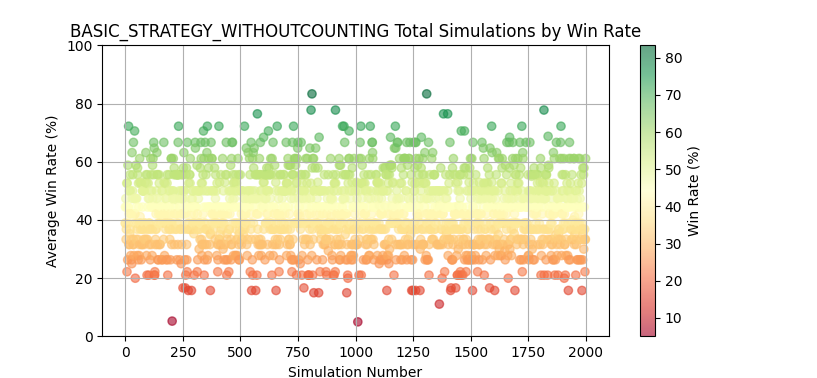
\includegraphics[scale=0.6]{figures/graphs/bswc_wr_ts.png}
\end{center}
\caption{Basic Strategy without Counting : Win rate x Total Simulations}
\label{fig:bswc_wr_ts}
\end{figure}

With respect to brute force models Basic Strategy without counting  shows a more concentrated distribution of win rates around 25-60\% as can be seen in Figure \ref{fig:bswc_wr_ts}. It performs quite like Always Hit model that we covered. But in basic strategy model that there are doubling involved in certain scenarios as a consequence of this this model may have more ROI in these cases. So let's examine the Money vs. Win Rate graph for the basic strategy model without counting to get better understanding in profitability of model:
 
\begin{figure}[h]
\begin{center}
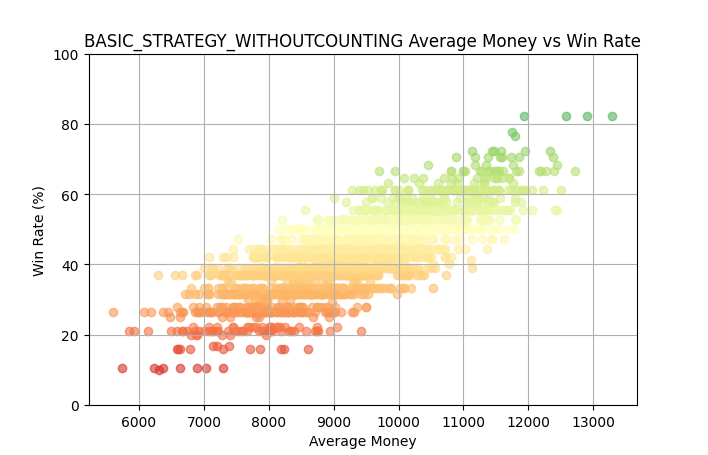
\includegraphics[scale=0.6]{figures/graphs/bswc_wr.png}
\end{center}
\caption{Basic Strategy without Counting : Money x Win Rate}
\label{fig:bswc_wr}
\end{figure}
\vskip\baselineskip

In the Figure \ref{fig:bswc_wr}, we observe that the basic strategy without counting resembles the Always Hit brute force graph but exhibits a higher maximum win rate and fewer low win rates. Although the majority of the games still fall on the unprofitable side, the basic strategy without counting performs almost as well as the Always Hit brute force model.

Let's now examine the ROI graph of the basic strategy without counting and compare it side by side with the Always Hit model. This comparison will provide a better understanding of the differences in their performance and profitability.

\begin{figure}[h]
    \begin{minipage}{0.45\textwidth}
        \centering
        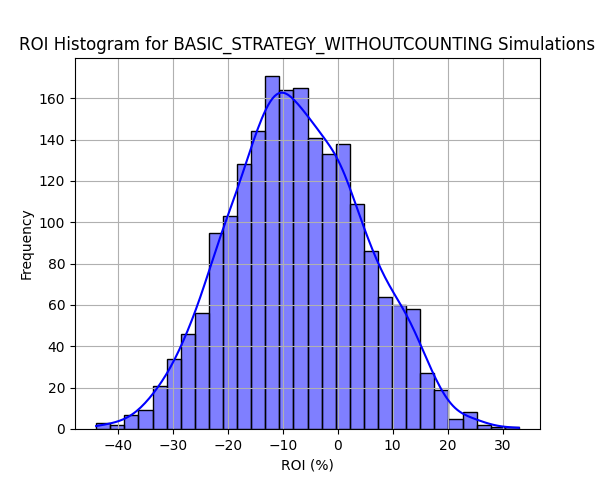
\includegraphics[scale=0.4]{figures/graphs/bswc_roi.png}
        \label{fig:ah_roi_left}
    \end{minipage}
    \begin{minipage}{0.45\textwidth}
        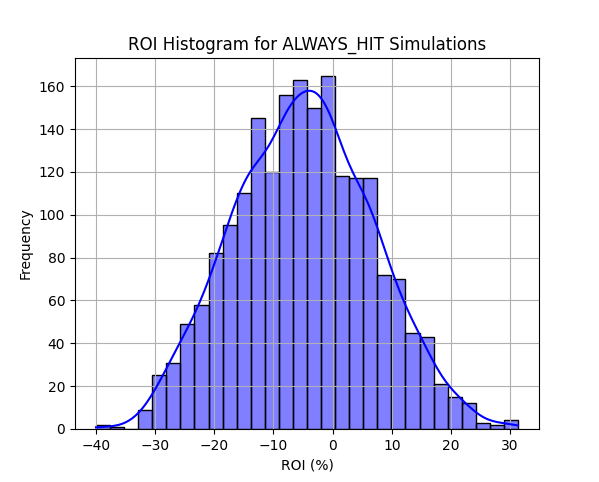
\includegraphics[scale=0.4]{figures/graphs/ah_roi.png}
        \label{fig:bswc_roi_right}
    \end{minipage}
    \label{fig:comparison_roi}
    \caption{Comparison between Basic Strategy without counting and Always hit model}
\end{figure}

We observe that there is not a significant difference in ROIs between these models based on Figure 5.13. In the basic strategy model, the 0-5\% ROI range is slightly steeper means that it has more neutral like ROIs compared to the Always Hit model, but the average ROI for both models is approximately the same.

\subsection{Basic Strategy with Counting}

In \ref{basic_strateg_with_counting}, we discussed the basic strategy with counting. The counting method is used in blackjack to adjust bets according to the calculated house edge in the current situation. By counting high and low cards and dividing by the remaining decks, we obtain the true count, which is then used to set the bet size.

Since adjusting bets is a fundamental aspect of this model, there are several situations that we might encounter. 

True count may increase a lot due to cards in the deck are nearing to end bet size can be increase in unwanted ways. In order to prevent this maximum bet in settings should be set advisedly. Even though a maximum bet size is set, the algorithm may still incur significant losses as the end of the deck approaches. This situation can arise because the true count can become highly volatile with fewer remaining cards, leading to larger swings in betting amounts and potential losses.

First, let's evaluate the performance of the basic strategy with counting in terms of win rate x total simulations done:

\begin{figure}[h]
\begin{center}
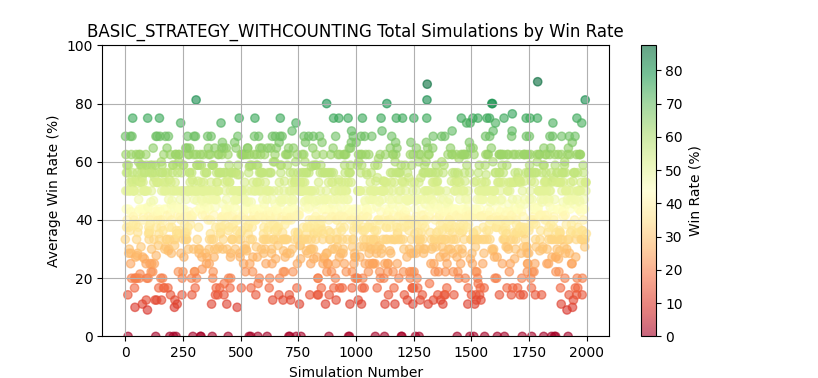
\includegraphics[scale=0.6]{figures/graphs/bsc_wr_ts.png}
\end{center}
\caption{Basic Strategy with Counting : Win rate x Total Simulations}
\label{fig:bsc_wr_ts}
\end{figure}

In the Figure \ref{fig:bsc_wr_ts} graph for the Basic Strategy With Counting model presents a more intriguing pattern compared to the other strategies. As mentioned above, model may act more unstable with respect to other models so this results in a noticeable presence of outliers, with some simulations showing win rates near 0\% (or 0), while others exhibit exceptionally high win rates. This variability indicates that while the counting strategy can lead to substantial gains under favorable conditions, it also introduces a higher risk of significant losses when the true count leads to larger bets. Bellow is the Money x Win rate graph of basic strategy with counting model, let's check how the unstability of the model effects money x win rate and ROI graphs.

\begin{figure}[h]
\begin{center}
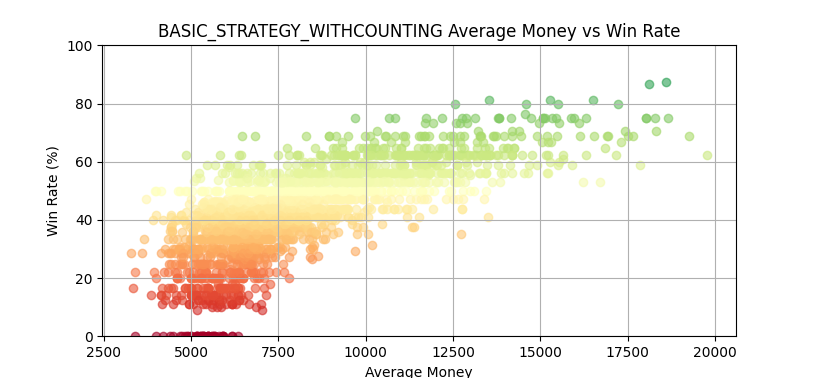
\includegraphics[scale=0.6]{figures/graphs/bsc_money_wr_big.png}
\end{center}
\caption{Basic Strategy with Counting : Money x Win Rate}
\label{fig:bsc_wr}
\end{figure}

At first glance, it is evident that there is a significantly higher number of simulations with win rates above 50\% in the Figure \ref{fig:bsc_wr}. The money axis is also wider, indicating that the counting technique allows the model to win more money by increasing bets when favorable conditions are detected. However, we also observe a considerable number of simulations with win rates in the 0-20\% range. This is due to the previously mentioned reason: when the true count becomes very high, the algorithm starts to bet excessively, which can lead to the player going bankrupt.

But aside from the losing cases ROI of this model may be higher than the others, because of the risking factor of the model. Lets see ROI table of it next:

\begin{figure}[h]
\begin{center}
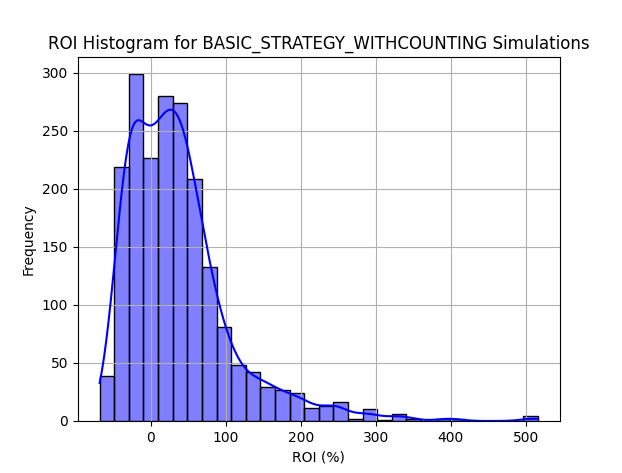
\includegraphics[scale=0.5]{figures/graphs/bsc_roi.png}
\end{center}
\caption{Basic Strategy without Counting : ROI x Frequencies}
\label{fig:bsc_roi}
\end{figure}

As clearly shown in Figure \ref{fig:bsc_roi}, the ROI of the basic strategy with counting model is significantly higher than the models we have discussed so far. The risk factor plays a crucial role here, as mentioned earlier. Playing with larger bets comes with greater responsibilities and potential for significant losses.

\section{Comparing Historical Data Model}
This method uses a database of past blackjack hands to inform the decision-making process, allowing the model to choose actions based on past results in similar situations. By examining this data, the model aims to mimic decisions that have previously led to positive outcomes.

The model may face limitations if the Historical Data does not adequately cover all possible game situations. In that case model is going to use basic strategy as we mentioned before.

Despite these challenges, the Historical Data model can offer significant advantages by using empirical evidence to guide decision-making. Let's check that how Historical Data performs in terms of win rate over simulations:

\begin{figure}[h]
\begin{center}
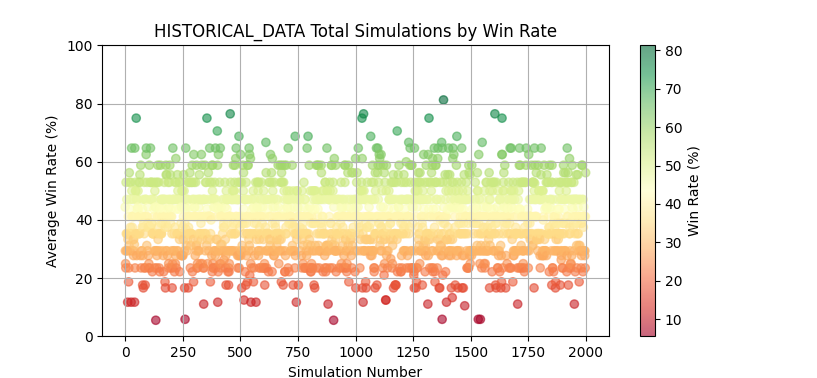
\includegraphics[scale=0.6]{figures/graphs/hd_wr_ts.png}
\end{center}
\caption{Historical Data : Win rate x Total Simulations}
\label{fig:hd_wr_ts}
\end{figure}

The graph for the Historical Data model in Figure \ref{fig:hd_wr_ts} indicates a distribution of win rates that closely resembles that of the Basic Strategy without Counting model. The win rates generally fall within the 20-50\% range, with a moderate number of simulations achieving win rates above 50\%. This similarity arises because the Historical Data model frequently resorts to basic strategy in the absence of sufficient Historical Data for specific scenarios. Consequently, the performance of the Historical Data model is highly dependent on the quality and coverage of the Historical Data. In simulations where the Historical Data is sparse or non-representative, the model defaults to basic strategy, resulting in win rates and performance metrics that align closely with those of the basic strategy without counting. Below is the Money x Win Rate graph of the Historical Data model:

\begin{figure}[h]
\begin{center}
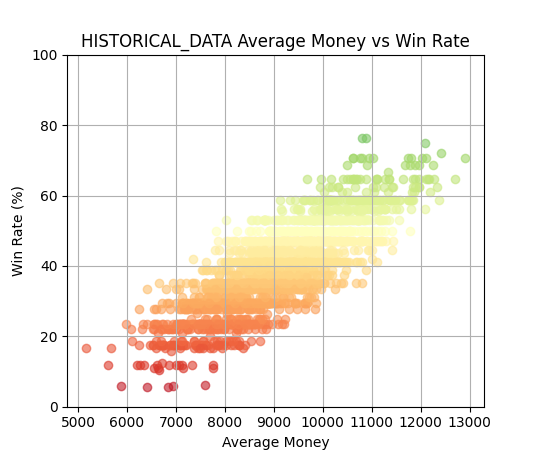
\includegraphics[scale=0.55]{figures/graphs/hd_wr.png}
\end{center}
\caption{Historical Data Model: Money x Win Rate}
\label{fig:hd_wr}
\end{figure}

As we can infer from the graph in Figure \ref{fig:hd_wr}, the Historical Data model does not perform as well as the basic strategy with counting. Its performance is approximately the same as the Always Hit model and the basic strategy without counting. One reason for this could be the nature of the Historical Data. In the 2000 games simulated, there may have been scenarios where the specific Historical Data was less applicable, causing the algorithm to default to the basic strategy. In fact, the ratio of calling the basic strategy within the 50 million hands dataset was 40\%. Therefore, it is normal for this model to resemble the basic strategy without counting.

In another set of 2000 simulations, the odds could be more favorable, and more historically accurate data could be used, potentially increasing the win rate. Conversely, the opposite could also occur, leading to a lower win rate.

Now, let's examine the ROI graph for the Historical Data model to better understand its profitability:

\begin{figure}[h]
\begin{center}
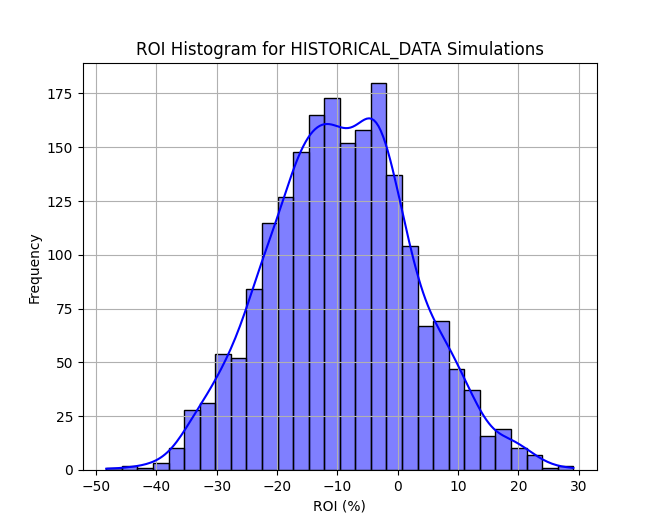
\includegraphics[scale=0.5]{figures/graphs/hd_roi.png}
\end{center}
\caption{Historical Data Model: ROI x Frequencies}
\label{fig:hd_roi}
\end{figure}

As mentioned before, it doesn't have a viable ROI to use this model in blackjack games. We can see in Figure \ref{fig:hd_roi} that in this 2000 simulations it has even lower ROI average then always hit model, which is a brute force model.

\section{Comparing RL (Reinforcement Learning) Model}

As mentioned in Chapter \ref{RL}, reinforcement learning (RL) is a sophisticated machine learning model that utilizes a learning algorithm, specifically Q-Learning in this instance, to make decisions and perform actions within an environment to maximize the "reward." In our application, we first create and train the RL model using various parameters. This pre-trained model is then used to simulate games, leveraging its learned experience to make optimized decisions. Unlike the other models we've discussed, which rely on fixed rules or Historical Data, the RL model continuously learns and evolves during its training phase, enabling it to make more informed and optimized decisions when applied in the game simulations. Given its extensive learning process and adaptability, we anticipate that the RL model will outperform the other models in terms of efficiency and profitability. 

Before delving into money x win rate and ROI graphincs lets first look at how well RL model will perform in terms of win rate x total simulations:
\vskip\baselineskip
\begin{figure}[h]
\begin{center}
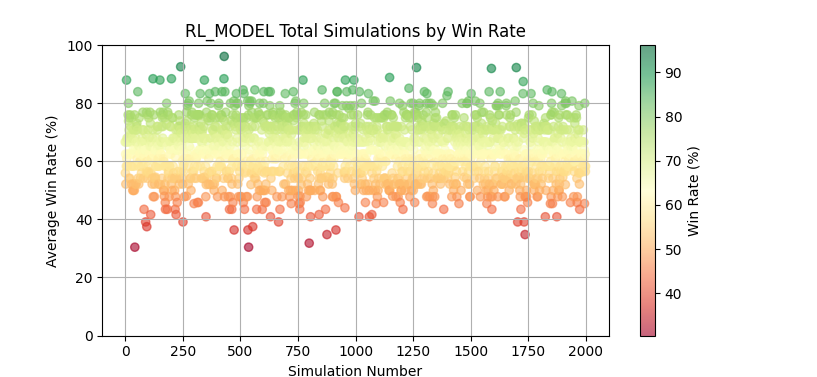
\includegraphics[scale=0.6]{figures/graphs/rl_wr_ts.png}
\end{center}
\caption{Historical Data : Win rate x Total Simulations}
\label{fig:rl_wr_ts}
\end{figure}
\vskip\baselineskip

The graph for the Reinforcement Learning (RL) model in Figure \ref{fig:rl_wr_ts} shows a higher overall win rate compared to other models. Most simulations achieve win rates in the 50-80\% range, with several exceeding 80\%. This indicates the RL model's superior learning capability and adaptability in optimizing decisions. The RL model consistently performs well, as reflected by the tight clustering of win rates around the higher percentages. This consistency and higher win rate make the RL model a promising approach for blackjack strategies. Now lets look at Money X Win Rate graph of Reinforcement Learning model in order to get more visual information about the models success:
\vskip\baselineskip

\begin{figure}[h]
\begin{center}
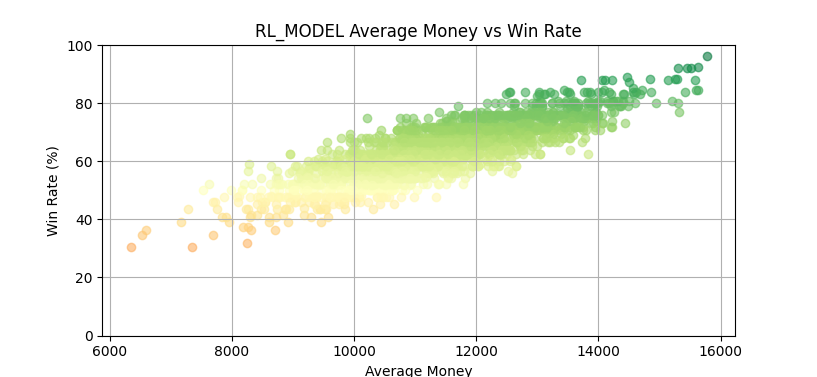
\includegraphics[scale=0.6]{figures/graphs/rl_money_wr_big.png}
\end{center}
\caption{Reinforcement Learning: Money x Win Rate}
\label{fig:rl_wr}
\end{figure}

\vskip4\baselineskip

We can clearly see from the Figure \ref{fig:rl_wr} that the RL model achieves significantly higher profitability compared to the other models. Remarkably, there are approximately 100 simulations with a win rate exceeding 80\%, as will be further illustrated in the ROI chart discussed next. On average, the majority of the simulations fall within the 55-65\% win rate range, which is still superior to any of the previously examined models. To ensure that these results are not merely due to favorable training conditions, we will generate additional charts with 2000 simulations at the end of this chapter to verify the consistency and reliability of the model's performance.

Let's now examine the ROI table to assess the consistency of the RL model in terms of returning the player's investment in the game:

\begin{figure}[h]
\begin{center}
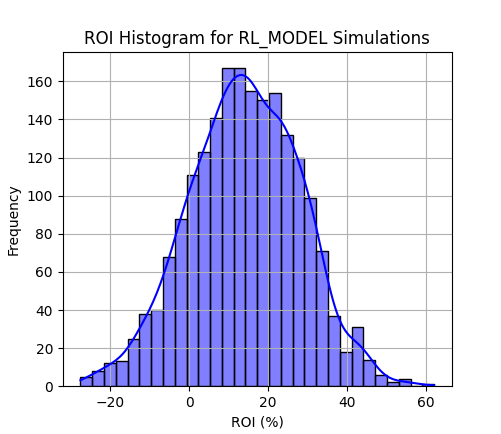
\includegraphics[scale=0.6]{figures/graphs/rl_roi.png}
\end{center}
\caption{Reinforcement Learning: ROI x Frequencies}
\label{fig:rl_roi}
\end{figure}

As shown in the figure \ref{fig:rl_roi}, demonstrates a notable consistency in the model's ability to return the player's investment. The majority of the simulations fall within the 0-30\% ROI range, with a prominent peak around the 15-20\% mark. This indicates that most of the simulations are profitable, providing a positive return on investment.


\begin{figure}[h]
    \begin{minipage}{0.45\textwidth}
        \centering
        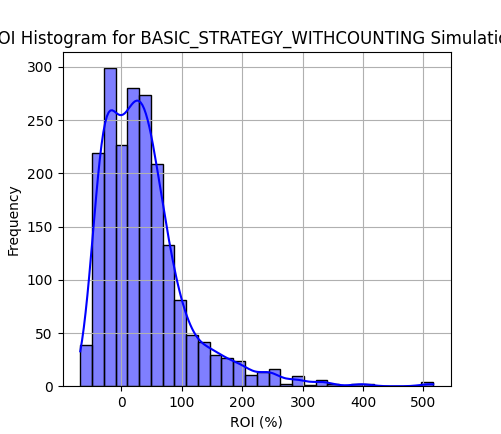
\includegraphics[scale=0.5]{figures/graphs/rl_vs_bsc_roi1.png}
        \label{fig:ah_roi_left}
    \end{minipage}
    \begin{minipage}{0.45\textwidth}
        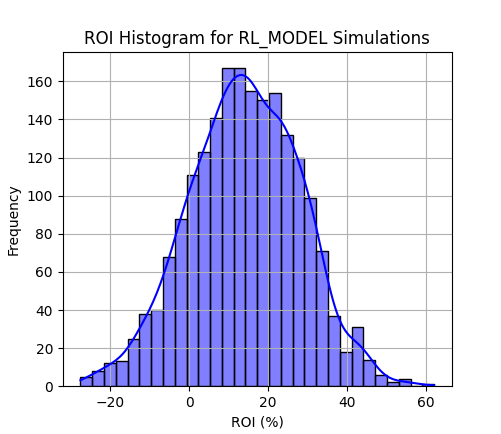
\includegraphics[scale=0.5]{figures/graphs/rl_roi.png}
        \label{fig:bswc_roi_right}
    \end{minipage}
\label{fig:comparison_roi}
\caption{Comparison between Basic Strategy with counting and Reinforcement Learning}
\end{figure}

In Figure 5.23, there is a comparison of models that have best ROI we gone trough. If we first check it by just the shape of it we can see that basic strategy without counting has more skewed graph, that has its peeks at -10-10\%'s with extending its ROI up to 500\% in some simulations which we can categorize them as outliers. On the other hand RL model histogram has much more symmetrical and bell-shaped graph, which suggests us that the RL model provides more consistent returns, with fewer extreme outliers.

The RL model has a small portion of simulations with negative ROI, but these are relatively few and less severe, mostly ranging between -20\% and 0\%. This indicates that the RL model has a lower risk of significant losses. On the contrary basic strategy with counting model, have negative ROI in graph (reaching from -40 to 0), might still present a risk due to the high variability in its returns, as indicated by the long positive tail.

The RL model demonstrates greater consistency and predictability in its performance. The narrow spread of ROI values around the peak indicates that simulations yield a similar range of returns, making it a more reliable model for consistent gains. But in basic strategy without counting with its wider spread and occasional high returns, suggests that while it can achieve very high returns in certain scenarios, it is less predictable and carries a higher variance in outcomes.

Overall, the RL model outperforms the both next best performed model basic strategy with counting model and the other models in terms of consistency and predictability, providing a more reliable and steady return on investment. The Basic Strategy with Counting model, while capable of achieving very high returns in some cases, exhibits greater variability and higher risk. 

\chapter{CONCLUSION}
\label{chapter:conclusion}

The comparative analysis of various blackjack strategies provides valuable insights into their performance and profitability. 

The brute force methods, including always hit, always stand, and random hit/stand, show fundamental differences in their win rates and ROI. Among these, the always hit strategy demonstrates the best performance, when its hit threshold set wisely, though it remains sub-optimal compared to more sophisticated models.

Basic strategy models, both with and without card counting, offer significant improvements over brute force methods. The basic strategy with counting model, shows higher win rates and potential for larger profits due to its adaptive betting strategy. However, this model also exhibits greater volatility, with notable outliers due to its aggressive betting behavior when the true count is high. The over-betting situation is also can be solved via setting a reasonable maximum bet size.

The reinforcement learning (RL) model stands out as the most consistent and profitable strategy. Trained using a variety of hyper-parameters, the RL model not only achieves high win rates but also maintains a balanced ROI across simulations. This consistency makes it a reliable choice for players seeking stable returns.

Historical data models, while informative, do not perform as well as the RL and counting strategies. Their reliance on past data leads to mixed results, with performance heavily dependent on the specific dataset used.

In summary, while the basic strategy with counting can achieve high returns in certain conditions, the reinforcement learning model proves to be the most effective overall, offering a balance of high win rates and consistent ROI. Further optimization of hyper-parameters could enhance the RL model's performance even more, solidifying its position as the best strategy for blackjack gameplay.

\section{Future Work}
Several enhancements and extensions can be implemented to improve the current system and provide a more comprehensive analysis of blackjack strategies:

\begin{itemize}
    \item {\textbf{User Interface Improvements:}} The GUI can be made more user-friendly and responsive, offering better feedback to users. For instance, incorporating sounds to notify users when simulations are complete would enhance the user experience.

    \item {\textbf{Graph Performance Optimization:}} The current graph creation screen can be slow when handling large datasets. For example, creating a graph with 2000 simulations, each with approximately 30 games, results in processing around 60,000 games, which can cause lag. Developing a custom graphing system could mitigate these performance issues.
    
    \item {Expansion of Brute Force Models:} New brute force models, such as "always doubling" or "imitate dealer/match dealer" \cite{paper:8} can be added to the system. Alternatively, these strategies can be integrated into existing models to provide a broader range of simulation options.
    
    \item {\textbf{Enhancements to Basic Strategy Models:}} Implementing features like insurance and surrendering could offer a more complete basic strategy model. Although these features may not significantly impact the results in 2000 simulations, their inclusion would provide a more accurate representation of real gameplay. Additionally, different counting strategies beyond the HI-LO method could be used, offering users the ability to select and compare various counting methods through the settings.
    
    \item {\textbf{Improvement of Historical Data Models:}} Access to better historical data would significantly enhance the accuracy and reliability of the historical data model. However, due to the restrictive nature of casinos regarding this information, obtaining such data may be challenging. If viable methods to access more comprehensive historical data are found, they should be increase the performance of the model.
    
    \item {\textbf{Advancements in Reinforcement Learning Models:}} The RL model can be further refined by incorporating additional actions, beyond just hit, stand, and doubling. Exploring other RL algorithms and comparing their performance could yield valuable insights. Additionally, a real-time learning model that updates based on the current data during gameplay could be developed.
\end{itemize}


\printbibliography

\appendix
\end{document}
